\documentclass[twocolumn]{article}
\usepackage[utf8]{inputenc}
\usepackage{graphicx}
\usepackage{float}

\title{Water Utility}
\author{Wen Ye, Gautam Agarwal, Bryan Jin}
\date{November 2020}

\evensidemargin=-0.5in
\oddsidemargin=-0.5in
\addtolength{\textwidth}{1 in}
\setlength\columnsep{30pt}
\setlength{\voffset}{-0.75in}
\textheight=650pt
\begin{document}

\maketitle

\section{Introduction}


 Much of Madison's water main infrastructure dates back to World War II and the immediate postwar era, when pipes were made of a less durable material called spun cast iron.(reference needed) As the pipes start to age, repair work for these pipes has increased drastically for the City of Madison Water Utility Crew, especially in the winter. Meanwhile, PILOT (Payment in Lieu of Taxes) made by the Madison Water Utility to the city of Madison is increasing over time because its amount is determined by the value of the utility's infrastructure and area property tax rates. As a result of water main repair work, PILOT amount would get greater. We care because PILOT is part of the water bill and every resident in Madison who uses water pays it. 
 
 Hence, we want to address the question: \textbf{what are the factors that influence the number of water main breakages and how do they affect it?} By answering this question, we hope to build a predictive model for the number of water main breakages in the city of Madison. 

As a separate topic, we also looked at water usage over the last two years. Specifically, we wanted to know: how has water usage changed from 2019 to 2020, possibly due to tumultuous events such as the pandemic and the subsequent lockdown?. Ideally, we would create a model that explains what factors affect water usage and use this model to predict water usage for the upcoming year.

\section{Utilization}

Figure \ref{fig:total_usage} compares total water usage between 2019 and 2020. The total water usage between 2019 and 2020 is very similar until around June 24. In particular, Wisconsin's stay-at-home order, which was announced around March 24, did not seem to have a noticeable effect on total water usage. 

On June 24, 2020, the total water usage plunged, and afterwards, the water usage in 2020 seems to exhibit a very different behavior from both the water usage in 2019 and the water usage in 2020 prior to June 24.

Figure \ref{fig:total_usage} poses two questions: why does the water usage level become erratic starting from late June 2020? Does water usage for specific classes (rather than just total water usage) show the same patterns?

\begin{figure}[H]
    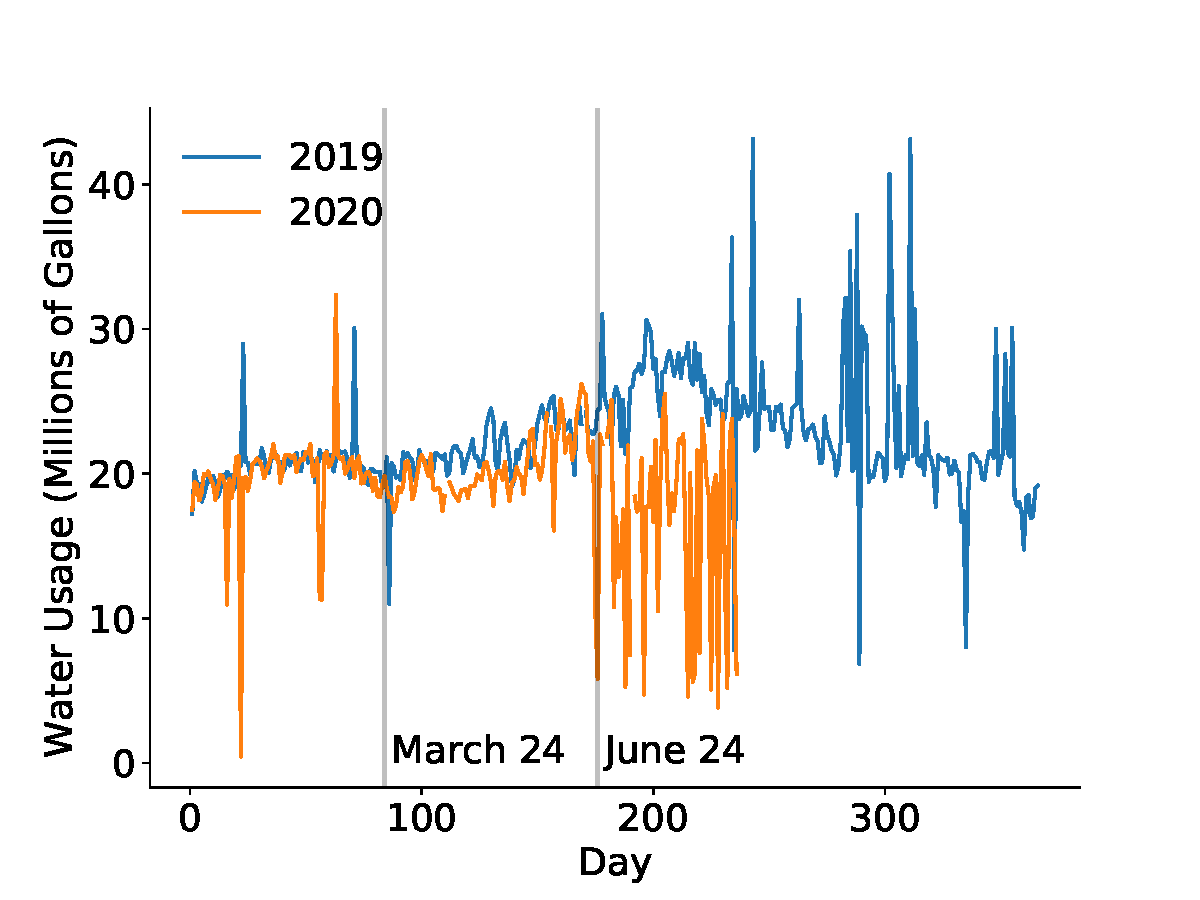
\includegraphics[width=\columnwidth]{Bryan/total_water_usage_new.pdf}
    \caption{Total Water Usage, 2019 vs. 2020}
    \label{fig:total_usage}
\end{figure}

Figure \ref{fig:water usage by category} attempts to address the second question. The plots show that a high variance pattern appears in each water usage category after June 24, 2020. 

By plotting each category separately and with its own scale for the $y$ axis, we highlight the fact that the pattern of increased variance after June 24 occurs in each category. The drawback of this approach is that visually comparing the line graphs with each other can lead to misleading results. For example, the industrial water usage graph seems to have greater variance across the year compared to the other categories, but this is because the $y$ axis range for Industrial is much smaller than for categories such as Total or Residential. 

We also observe patterns in the Figure \ref{fig:water usage by category} plots that were not discernible when we only looked at total water usage. For example, commercial water usage does show a decrease around March 24, which makes sense: the rise of COVID correlates with a decrease in commercial water usage. Interestingly, public authority water usage increases right after March 24. 


\begin{figure*}
    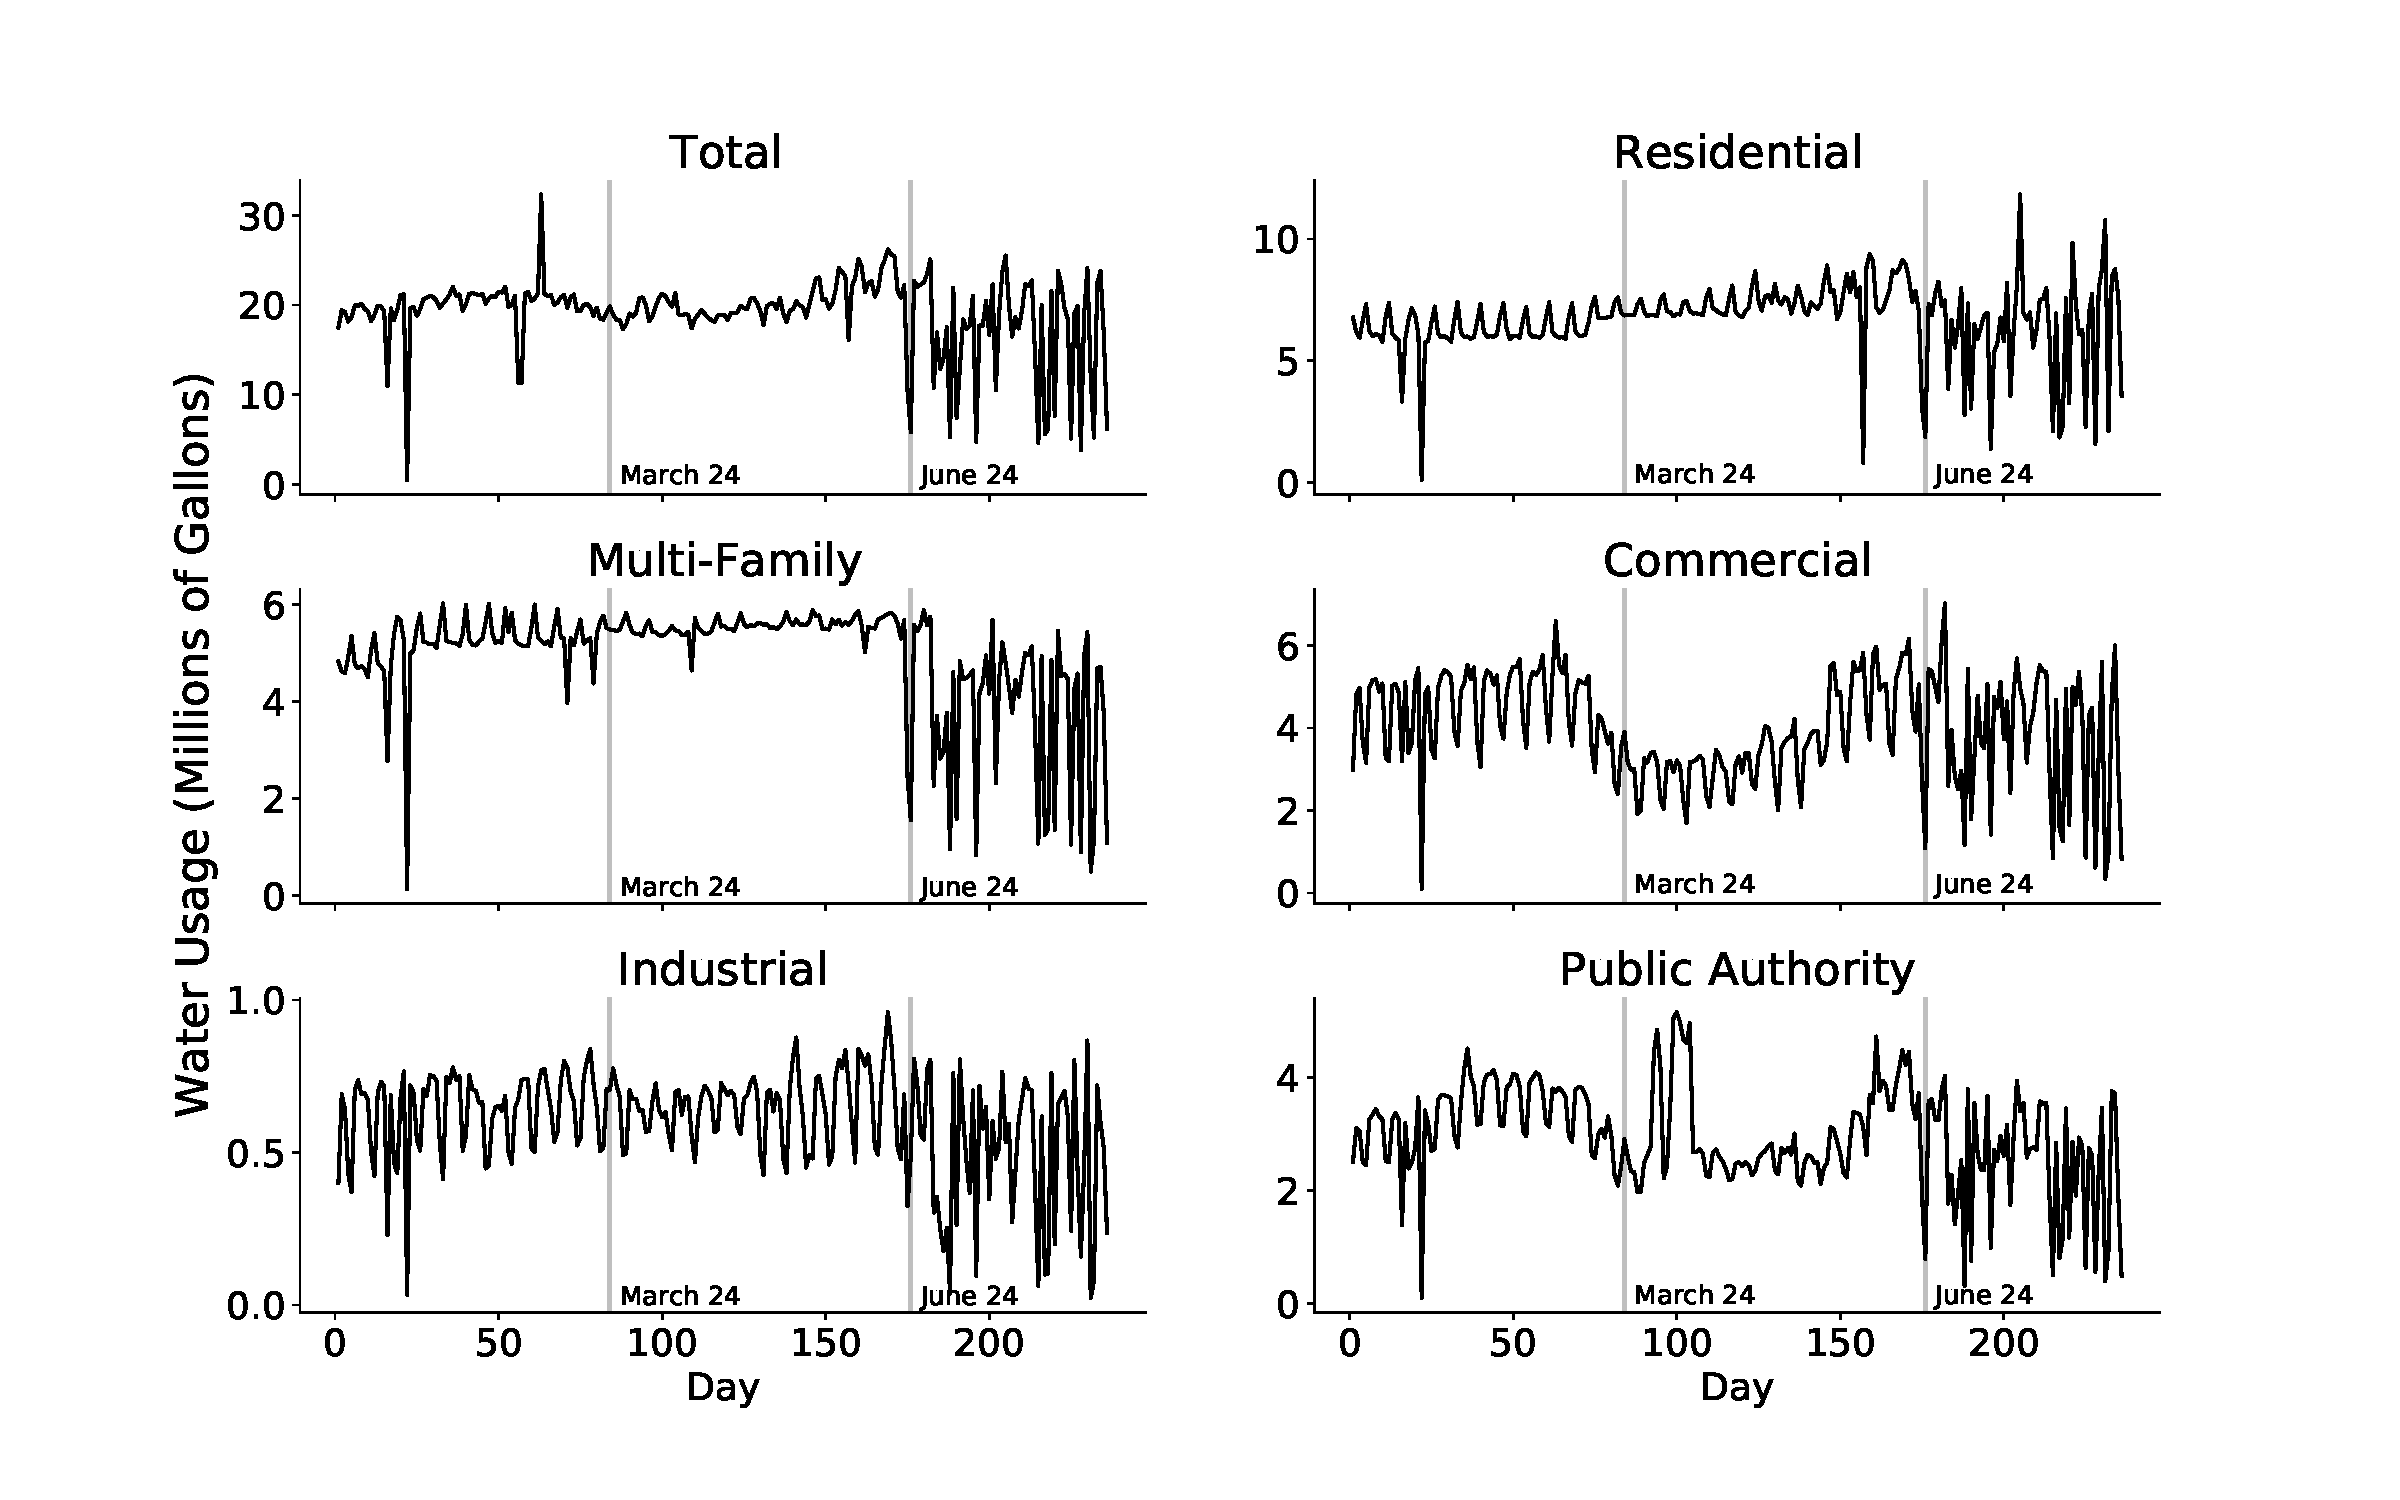
\includegraphics[width=\textwidth]{Bryan/all_water_usage_2020.pdf}
    \caption{2020 Water Usage by Category}
    \label{fig:water usage by category}
\end{figure*}




\section{Breakage Factors}


\subsection{Season and Temperature}

Figure \ref{fig:Hi} shows the total number of water main breaks by month from 1980 to 2020. The total number of water main breaks substantially increases in the months of December, January and February which is the winter season. Low temperatures and other winter conditions may contribute to this apparent difference in the number of breaks between different months of the year. From this plot, we decide to examine more closely the relationship between temperature and the number of breaks. 

\begin{figure}[H]
    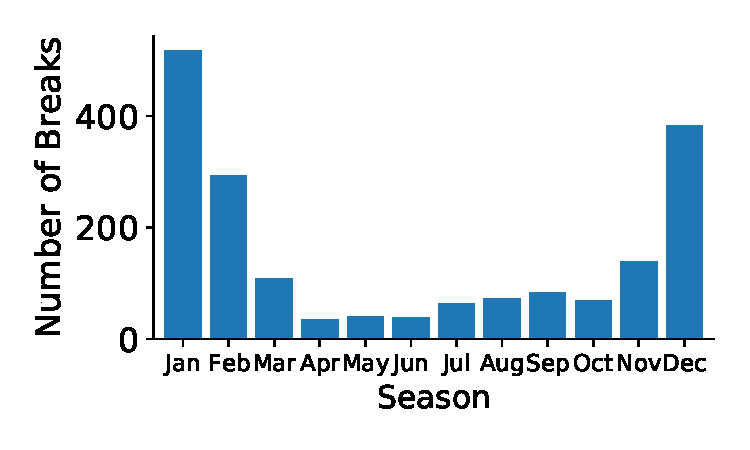
\includegraphics[width=\columnwidth]{Wen/breaks by month.pdf}
    \caption{Number of Water Main Breaks by Month}
    \label{fig:Hi}
\end{figure}


Figure \ref{fig:min temp and counts} compares the minimum temperature and the number of water main breaks for each year (again from 1980 to 2020). The minimum temperature of each year is scaled by 5 to make the peaks and dips more visible. Generally, peaks in the number of breakages correlate with dips in the minimum temperature. 

\begin{figure}[H]
    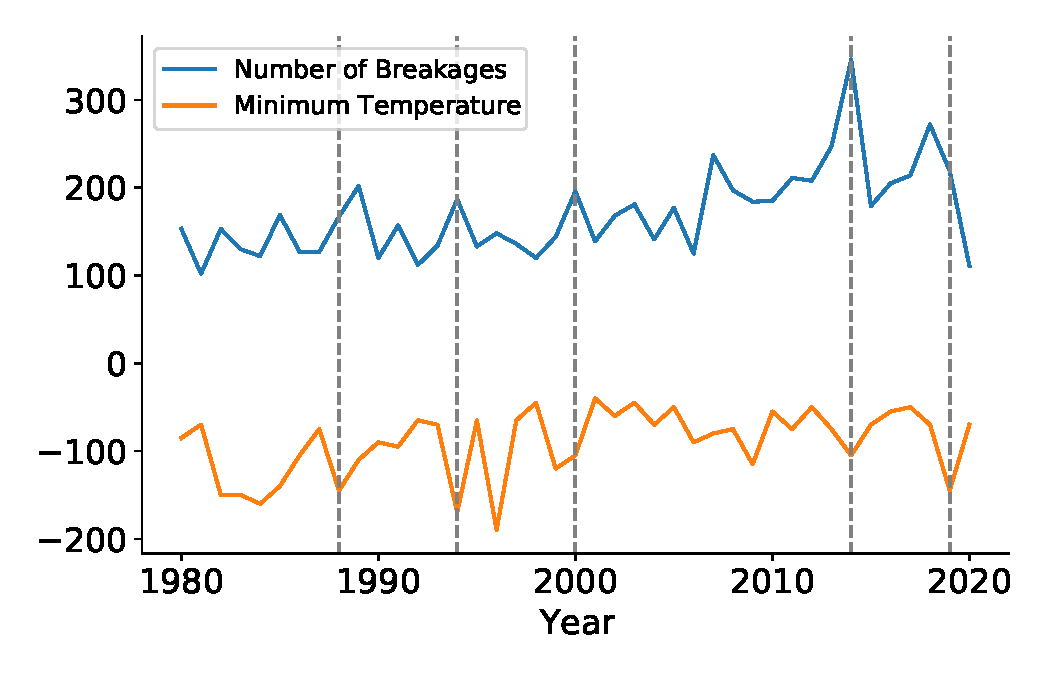
\includegraphics[width = \columnwidth]{Wen/min temp and count comparison.pdf}
    \caption{Comparison Between Min Temp and Breaks}
    \label{fig:min temp and counts}
\end{figure}

\begin{figure*}
    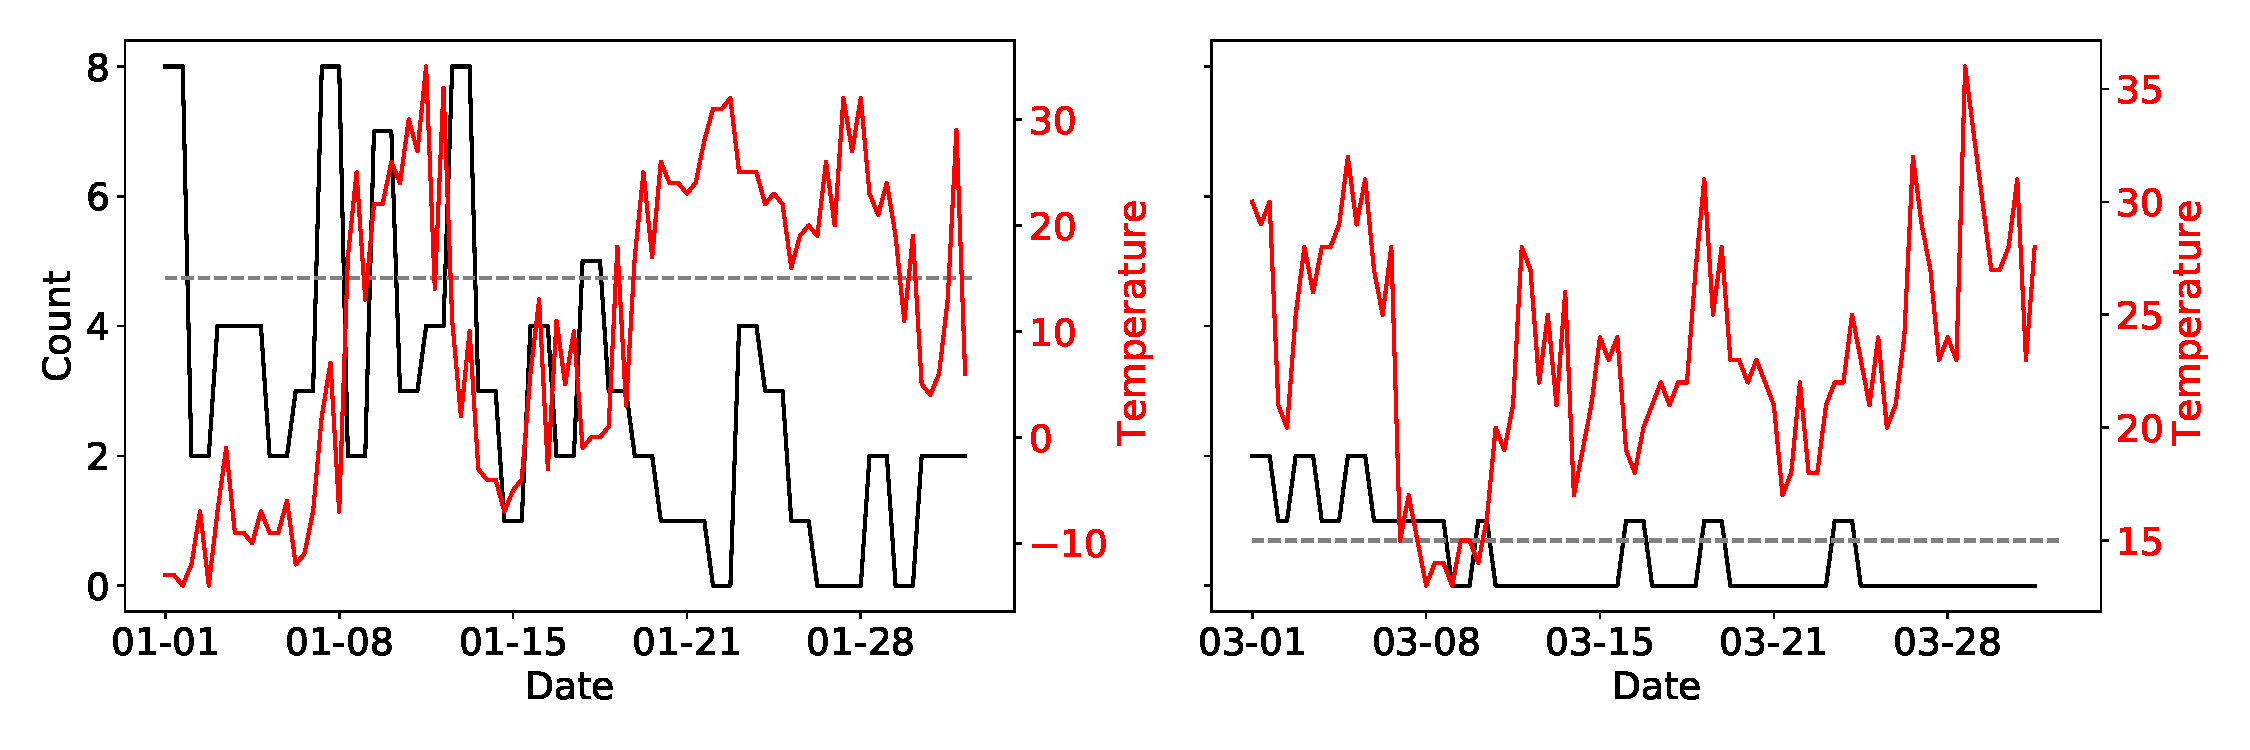
\includegraphics[width = \textwidth]{Wen/jan mar 2018 comparison.pdf}
    \caption{Jan and March comparison}
    \label{fig:comparison}
\end{figure*}

Figure \ref{fig:comparison} gives a more detailed comparison to tease out the influence of temperature and season. If we look at 15 Fahrenheit for January and March 2018, the month of March has 1 break on that day while the month of January has 7 breaks on the day with the same temperature. Here, we can infer that season is more influential in determining the number of breaks than the minimum temperature of the day itself. Meanwhile, examining the day of Jan 7th and Mar 18th, there's a significant sudden increase in temperature and the number of breakages went up alongside. This suggests that a sudden increase in temperature which could cause the soil to thaw too quickly is a contributing factor to breakages. 

\subsection{Pipe Depth}

\textbf Figure \ref{fig:Pipe Depth} describes the distribution of water main breaks with respect to the depth at which the main's pipe was laid. The cumulative frequency is 0.1 for pipes with depth at most 5 feet and 0.9 for pipes with depth at most 7 feet. This means 80 percent of water mains that break are laid 5-7 feet deep.

This may be because:

1.	It is most common for pipes to be laid at this depth

2.	Pipes that are laid at this depth are the most vulnerable to break

\begin{figure}[H]
    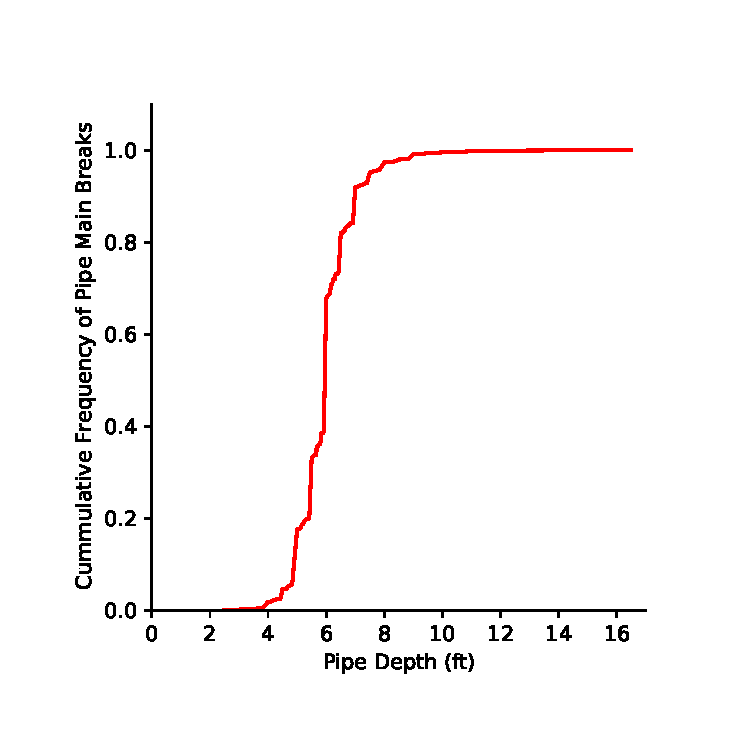
\includegraphics[width=\columnwidth]{Gautam/depth_cdf.pdf}
    \caption{Cumulative Frequency Distribution of Breaks by Pipe Depth}
    \label{fig:Pipe Depth}
\end{figure}


\subsection{Pipe Size}

\textbf Figure \ref{fig:Pipe Size} describes the distribution of water main breaks with respect to the size of the main's pipe. Most pipes that break are 5-6 metres long.

This may be because:

1.	It is most common to use pipes of this length

2.	Pipes of this size are the most vulnerable to break


\begin{figure}[H]
    
    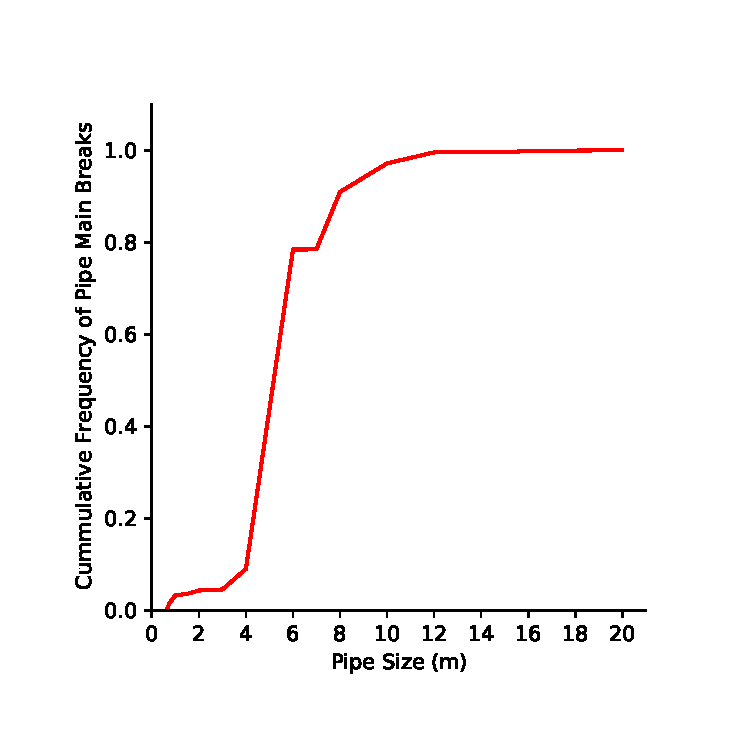
\includegraphics[width=\columnwidth]{Gautam/size_cdf.pdf}
    \caption{ Cumulative Frequency Distribution of Breaks By Pipe Size}
    \label{fig:Pipe Size}
\end{figure}

\subsection{Location}

\textbf Figure \ref{fig:Location} shows the geographic distribution of water main breaks for every decade. The number of breaks away from the inner city/downtown area have started to increase between 2000-2009 and 2010-2020. One possible explanation is the increasing population outside of the downtown area in the past 20 years. We also noticed that the number of breaks increase every decade.


\begin{figure*}
    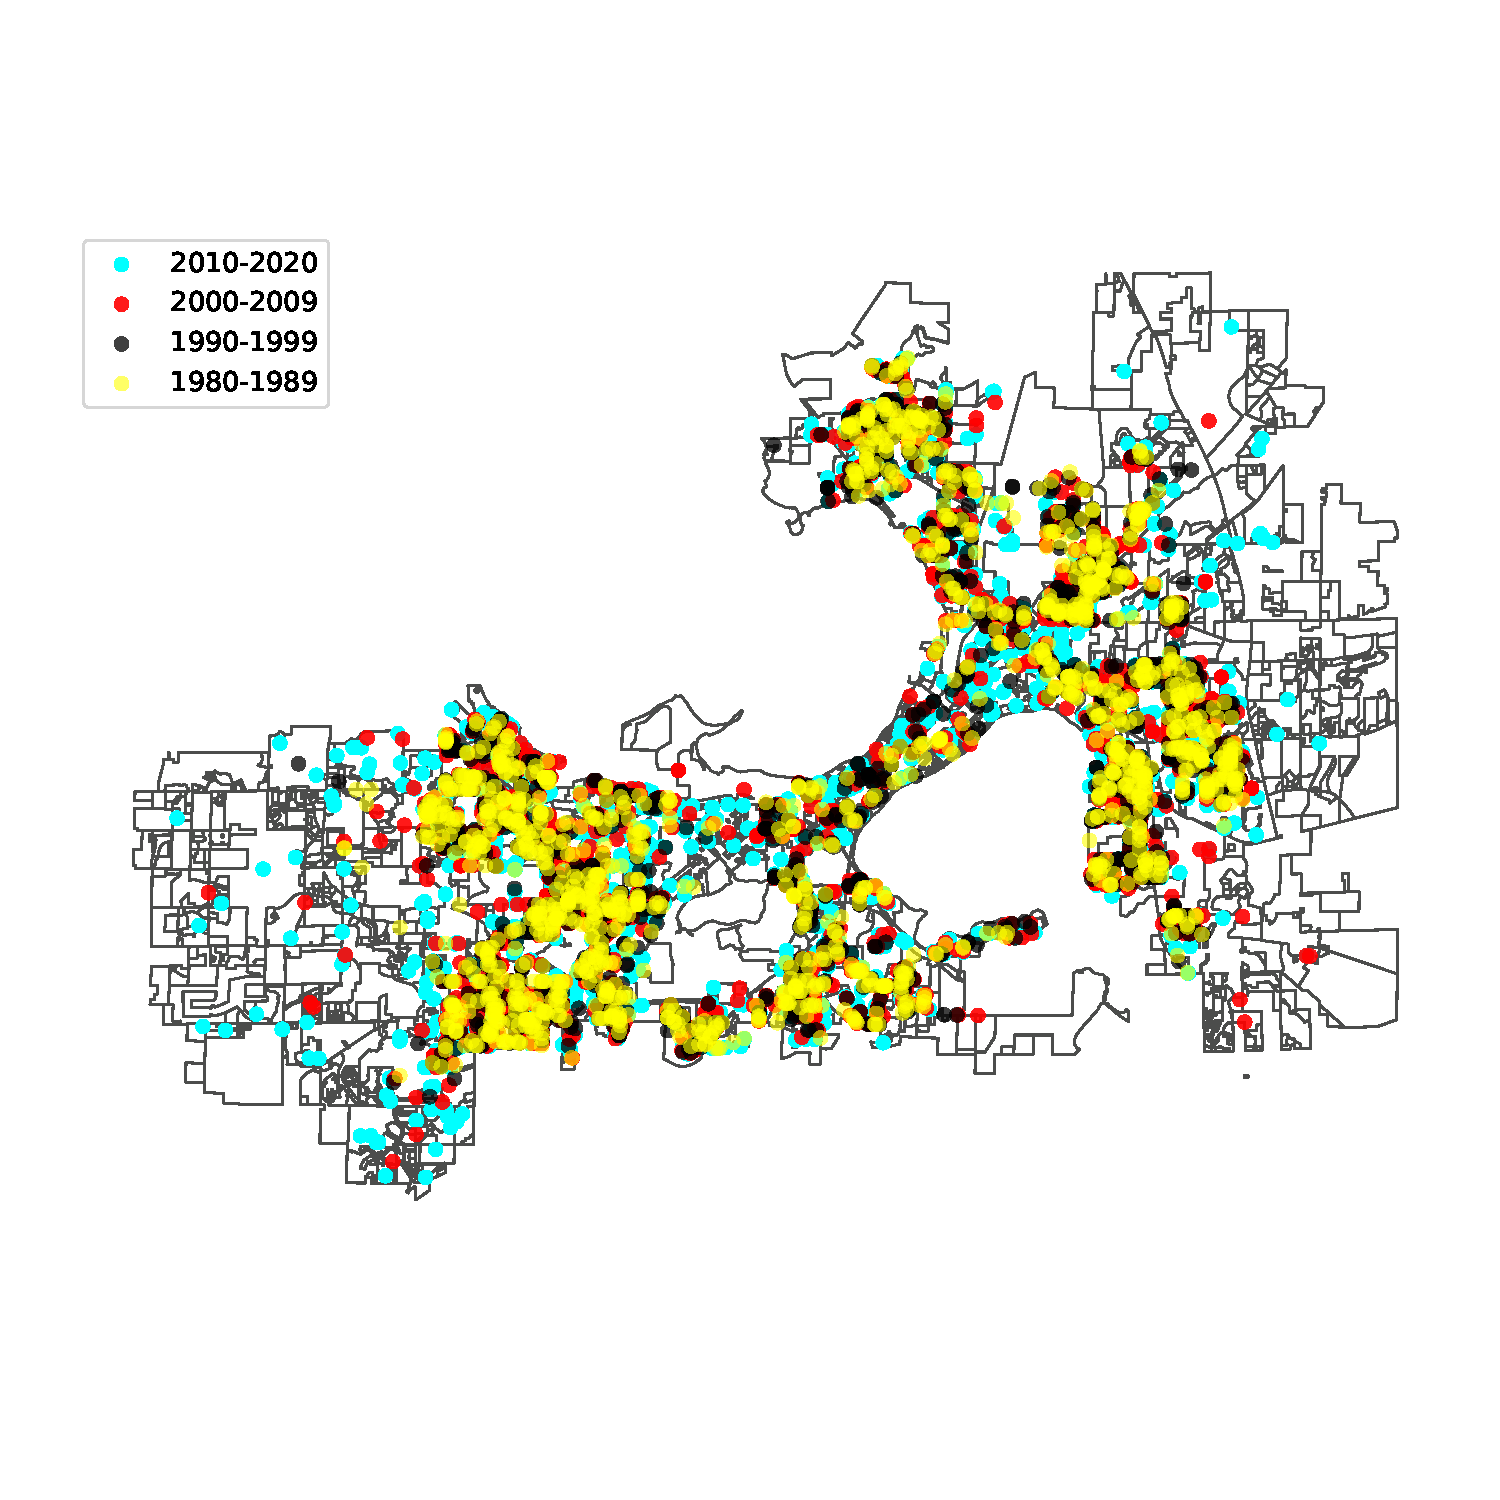
\includegraphics[scale=0.728]{Gautam/decade_plot.pdf}
    \caption{Pipe Main Breaks In City of Madison Every Decade}
    \label{fig:Location}
\end{figure*}


\subsection{Soil Type}

For the soil type variable, many water mains had a singular soil type: clay, sand, gravel, etc. Other water mains had two soil types: clay and sand, sand and gravel, etc. A few water main breaks even had three soil types: clay, sand, rock or clay, gravel, rock. The most common soil types were clay, sand, gravel, dirt, and rock. 

To get a better understanding of the soil type variable, Figure \ref{fig:One vs. Many Soil Type} shows how often the most common soil types appeared on their own vs. in combination with other types. For example, the leftmost bar shows that clay often appeared as the only soil type, while the rightmost bar shows rock mostly appeared with other soil types (such as sand and rock or clay and rock).

\begin{figure}[H]
    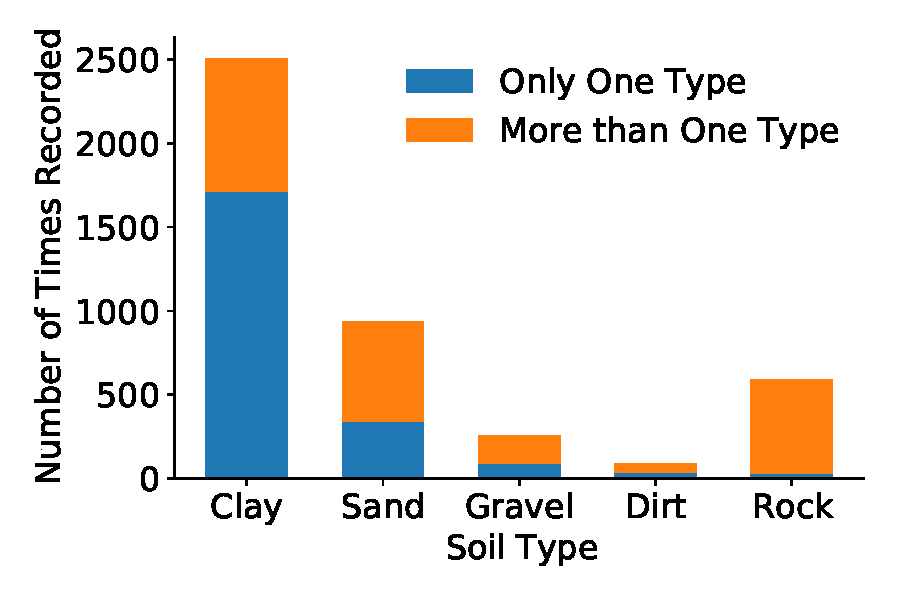
\includegraphics[width=\columnwidth]{Bryan/one_vs_multiple_soil_types.pdf}
    \caption{One Soil Type vs Multiple Soil Types}
    \label{fig:One vs. Many Soil Type}
\end{figure}

Figure \ref{fig:Soil Type Pairs} focuses on the instances of the soil type variable where two soil types are recorded. The leftmost bar shows that when clay appears as one of two types, the other type is most likely either sand or rock. Note that the three bars on the right indicate that when gravel, dirt, or rock appear in a pair, they are always paired with clay or sand. 

Overall, clay and sand seem to be the main soil types. Gravel, dirt, and rock seem to function as secondary soil types that can be associated with either clay or sand. To better understand the soil type variable, we may investigate how soil type relates to other variables such as location or pipe dimensions.

\begin{figure}[H]
    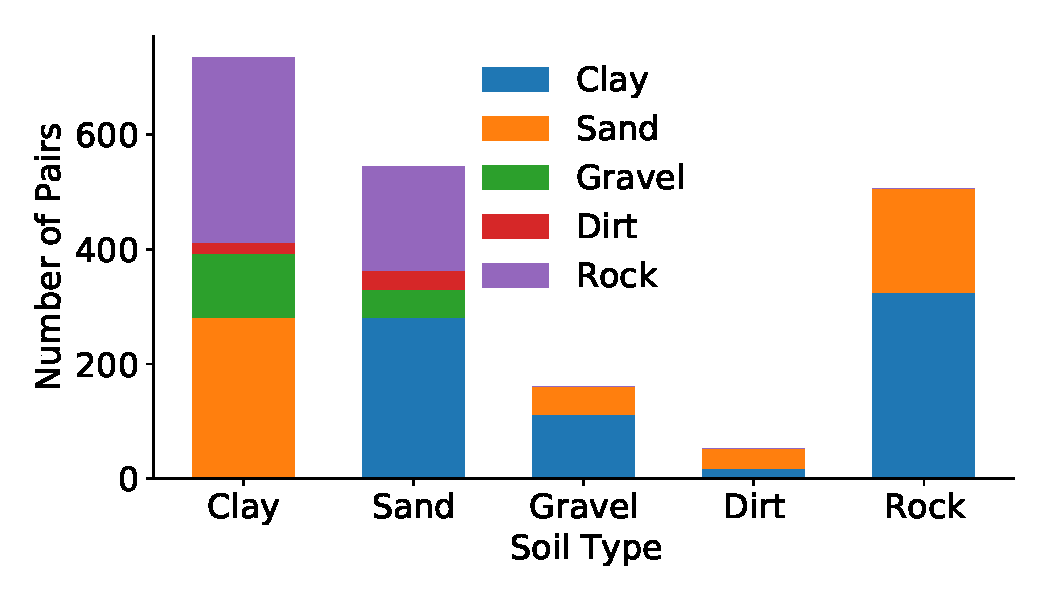
\includegraphics[width=\columnwidth]{Bryan/soil_type_pairs.pdf}
    \caption{Common Pairs of Soil Types}
    \label{fig:Soil Type Pairs}
\end{figure}



Fig \ref{fig:Soil Type and Season} shows the number of breakages by soil type in each season. The soil types are stacked in the order of the most number of breakages to the least. Clay has the highest number of breakages and Mud/Dirt has the lowest. Relative to Summer, breaks in rock/stone are up by 856\% during winter, whereas breaks in gravel are only up by 54\%. For all the soil types, rock/stone has the greatest increase in number of breaks and gravel has the lowest. It could be inferred that gravel is more resistant to Winter than all the other soil types and implementing new water main pipes in gravel in the future could reduce the number of breakages.

\begin{figure}[H]
    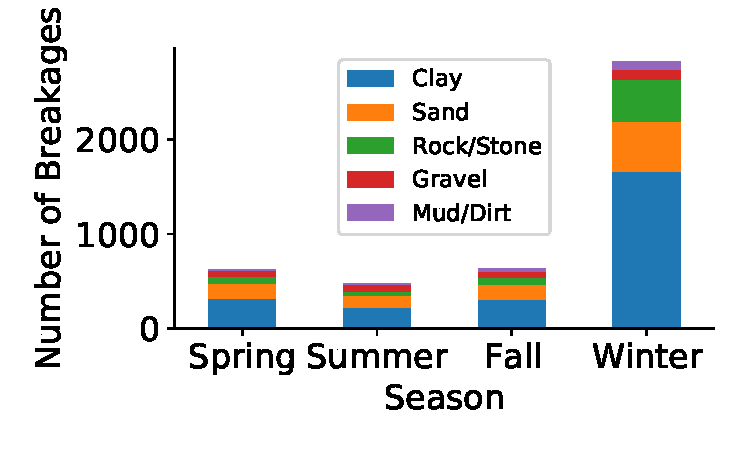
\includegraphics[width=\columnwidth]{Wen/Soil Type by Season.pdf}
    \caption{Percentage of Breaks by Season}
    \label{fig:Soil Type and Season}
\end{figure}


\begin{figure*}
    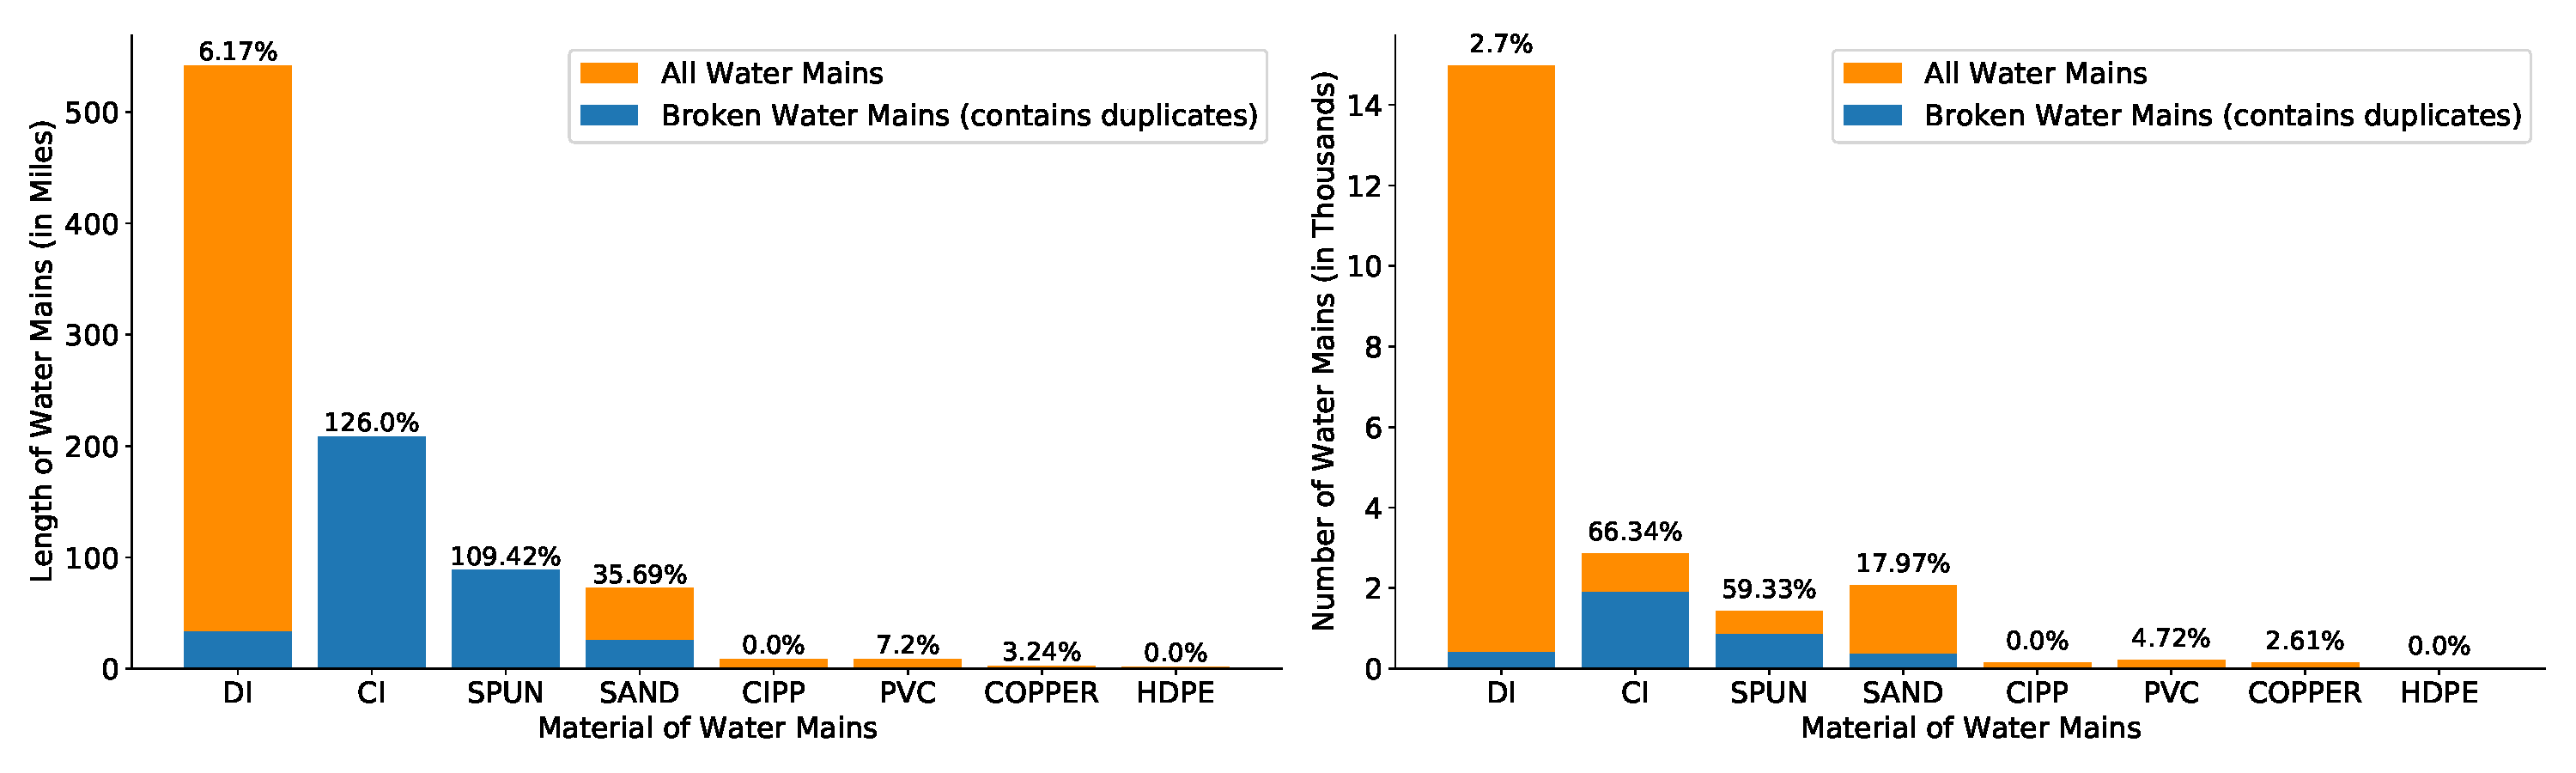
\includegraphics[width=\textwidth]{Wen/Material by len and count.pdf}
    \caption{Material of Water Mains}
    \label{fig:Material of Water Mains}
\end{figure*}
\subsection{Material Used}



Metal pipes are the most common type of water pipes, especially iron. In the city of Madison, 97.52\% of pipes are made of some variety of iron and these pipes are responsive for 99.6\% of breaks.  Most Iron pipes are used for pipes laid underground and copper pipes are used to connect water mains with buildings like households or public facilities and are relatively shorter in length compared to underground iron pipes. For iron pipes, Cast Iron (CI) pipes are used the most often for pipes laid at earlier eras because manufacturing and installation were relatively simple. The disadvantage is that CI pipes are brittle and vulnerable to temperature change which makes a big difference for cities in the North like Madison. On the other hand, Ductile Iron pipes are stronger in terms of both strength and resistance to weather as we'll see later in this section. (TODO: reference needed)


Fig \ref{fig:Material of Water Mains} gives a detailed breakdown of materials used for water pipes  in the city of Madison. The percentage on top of each bar is the rate of breaking.  From looking at the count of water mains plot alone (on the right), we can see that even though there are many pipes made of  Ductile Iron (DI), it has a low rate of breakages whereas CI and SPUN have rates of breaking greater than 50\%.Meanwhile, looking at the length of water mains, we see that CI and SPUN water mains have the percentage of breakage in terms of length higher than 100\%. But we know from the plot on the right that not all CI and SPUN pipes have broken. So, it can be inferred that some CI and SPUN pipes broke extensively. 

 \textbf{[BEGIN Wen 11/16]} 
Fig \ref{fig:Average Broken Length of Water Mains by Material} shows the Average Broken Length (in Feet) of Water Mains by Material. Just like the pattern we see from fig \ref{fig:Material of Water Mains}, among the iron types, even after we break down to a much smaller scale, CI pipes breaks the most followed by SPUN pipes. Moreover, looking at fig \ref{fig:Material of Water Mains}, there are about the same number of DI and SAND pipes broken. And in fig ref\ref{fig:Average Broken Length of Water Mains by Material}, The average broken length per week is slightly higher for DI pipes than SAND pipes. This might be that in general, when DI pipes were implemented, they were longer in length. 

\begin{figure}[H]
    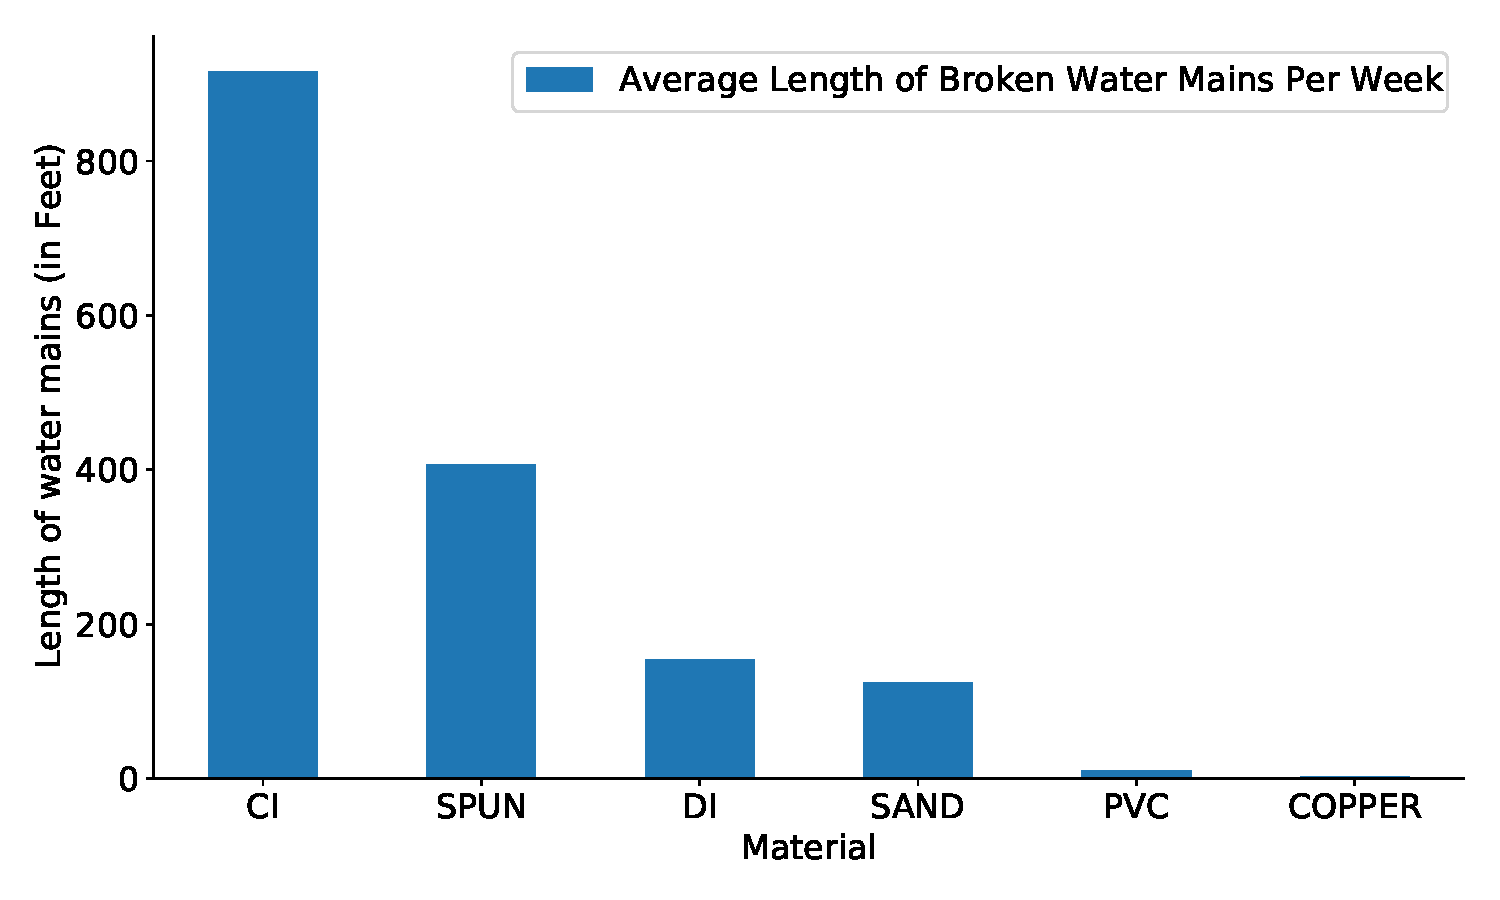
\includegraphics[width=\columnwidth]{Wen/Average Length of Broken Water Mains Per Week.pdf}
    \caption{:Average Broken Length of Water Mains by Material}
    \label{fig:Average Broken Length of Water Mains by Material}
\end{figure}
We next wanted to examine the change of average Broken Length of Water Mains over time. Fig \ref{fig:Average Broken Length of Water Mains by Iron Types over time} shows this change over time. The first thing that stood out was that pipes made of all iron types dipped together around 2005 and 2006 where the average broken length per week dropped to something close to 0. In trying to find out the reason behind this, we plotted this change over time against the temperature of that year and the temperature of 2005 and 2006 are within normal fluctuations of temperature. And the fact that CI pipes which stays high above all the other iron type pipes throughout the decades dipped to the same level as all the other iron types pipes lead us to think that there were some data recording issues during 2005 and 2006. 
\begin{figure}[H]
    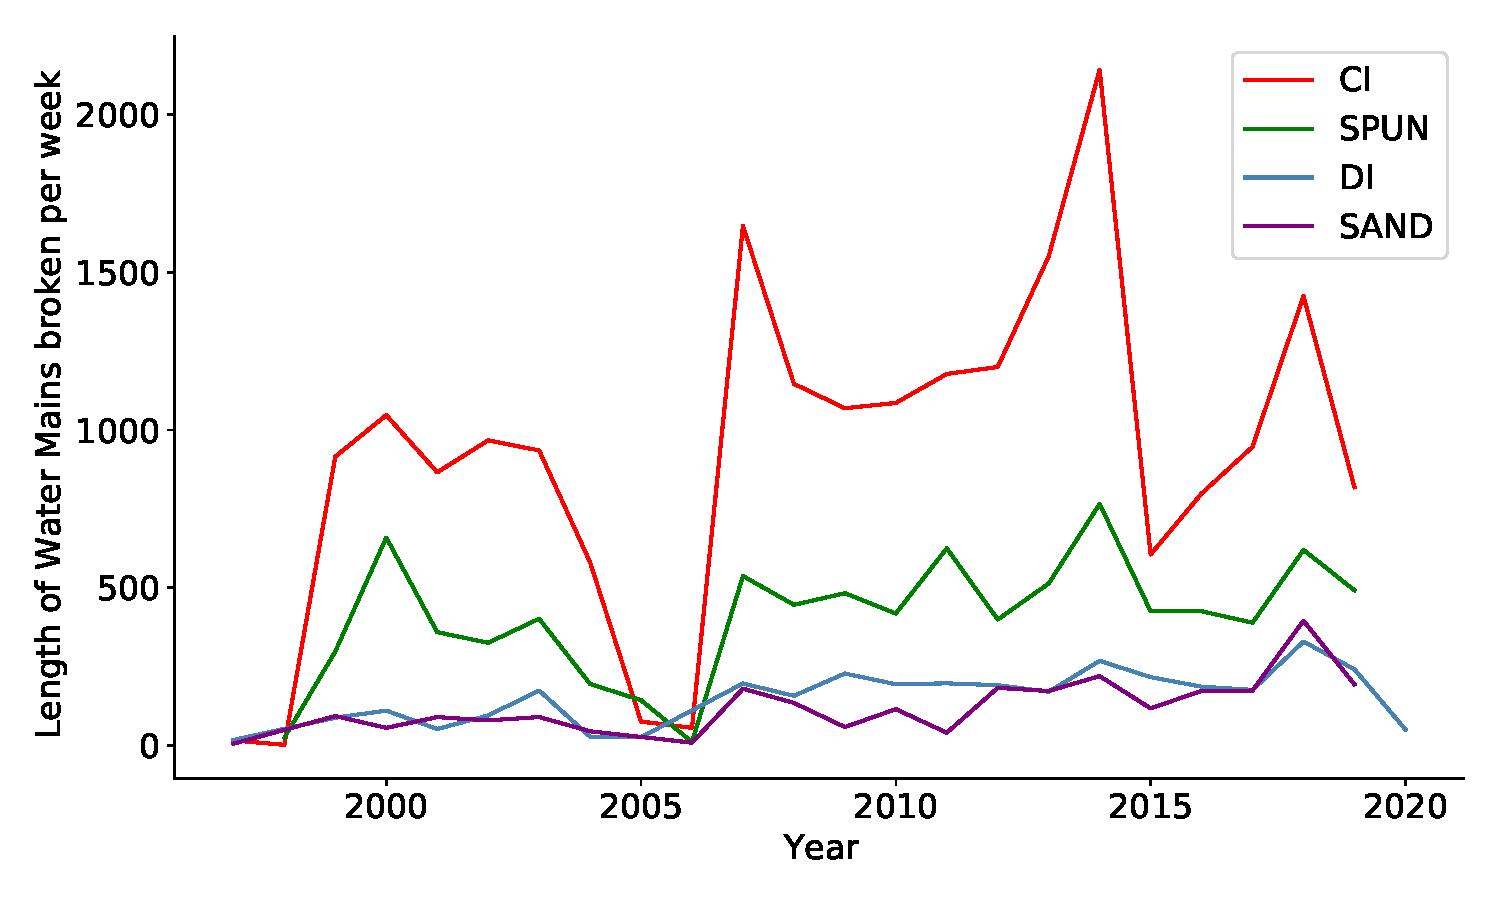
\includegraphics[width=\columnwidth]{Wen/ave broken len per week.pdf}
    \caption{:Average Broken Length (in Feet) of Water Mains by Iron Types Over Time}
    \label{fig:Average Broken Length of Water Mains by Iron Types over time}
\end{figure}
On the other hand, fig \ref{fig:Average Broken Length of Water Mains by Iron Types over time} also did not support the hypothesis that DI pipes were naturally longer than SAND pipes when implemented because when we break down to year by year, DI and SAND pipes really are staying at the same level. 
\textbf{[END]} 

Fig \ref{fig:Material and Season} shows the number of pipe breakages by different types of iron used separated into each season. The legend shows the percentage of increase in breakages in Winter compared to Summer. There's a drastic increase in the number of pipe made of CI and SPUN breaking in the Winter. In fact, CI and SPUN both went up by 953\% in Winter relative to Summer. Meanwhile, Sand Cast Iron(SAND) and DI have both a low rate of breaking as well as a smaller increase in breakage rate from summer to winter. 
\begin{figure}[H]
    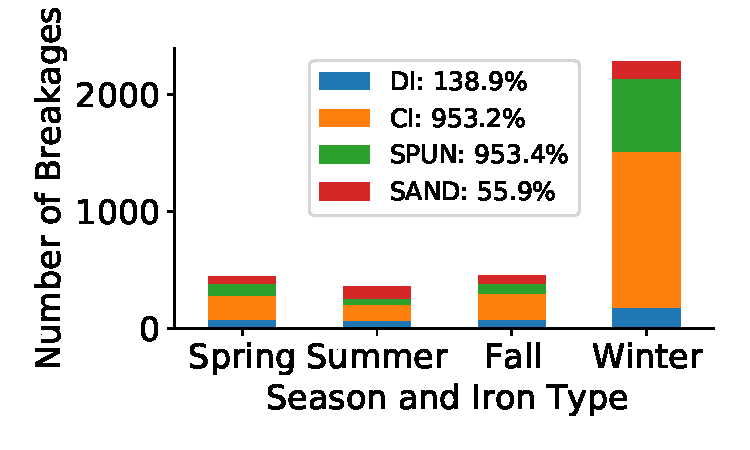
\includegraphics[width=\columnwidth]{Wen/Season and Iron Type.pdf}
    \caption{Material and Season}
    \label{fig:Material and Season}
\end{figure}
Looking at the two plots together,  it's reasonable to suggest that cutting the usage of CI and SPUN pipes can reduce the number of breakages. DI will be better choices. Pipe replacement is definitely a continuing process but to conclude for this section, the city should consider replacing CI and SPUN pipes before SAND pipes with DI pipes. 





\subsection{Pipe Life}

\textbf{[BEGIN Gautam 11/16]}

Figure \ref{fig:Material vs Lifetime} plots the cumulative distributive frequency of the number of pipe mains that have broken at least once, against their lifetime. These pipe are further differentiated by their material.

Here lifetime is defined as the time in years of the pipe mains from the time it was first installed to the time it was broken for the first as well as the second or third time. The pipes that do not break are not portrayed here.

 In the figure, it can be observed that majority CI pipes have a lifetime of 50 years, while SPUN pipes last 60 years. Some Sand pipes are used since World War 1 while the lifetime of DI pipes is low, with a maximum of 50 years. Data about copper breakages can be observed at a lifetime of 60 years with about 50 breakages.  

\begin{figure}[H]
    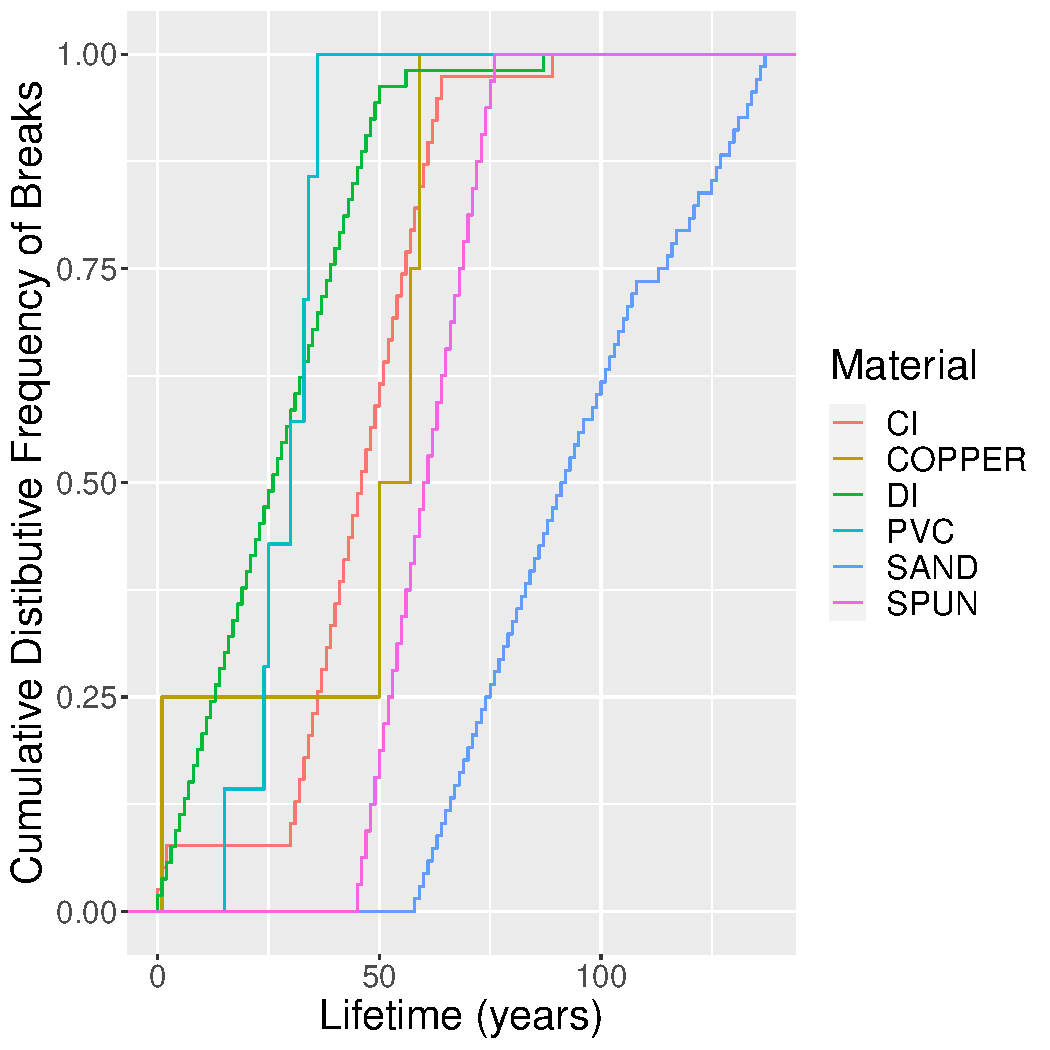
\includegraphics[width=\columnwidth,height=200px]{Gautam/lifetime.pdf}
    \caption{Lifetime for pipes of each material}
    \label{fig:Material vs Lifetime}
\end{figure}

\textbf{[END Gautam]}


\section{Modeling Breaks}


\subsection{Visualizing seasonal changes}

Before building a model to predict the number of breakages, we first want to know if the four seasons actually have distinct patterns in terms of the number of breakages. And Figure \ref{fig:Break Pattern by Seaon} shows that they indeed do. The range of temperature varies as well as the maximum number of breakages reached. The number of breakages is always an integer, but to reduce overlapping and have a better sense of where all the points lie, we added a little noise with a normal distribution centered at 0 and standard deviation of 0.1. 

\begin{figure}
    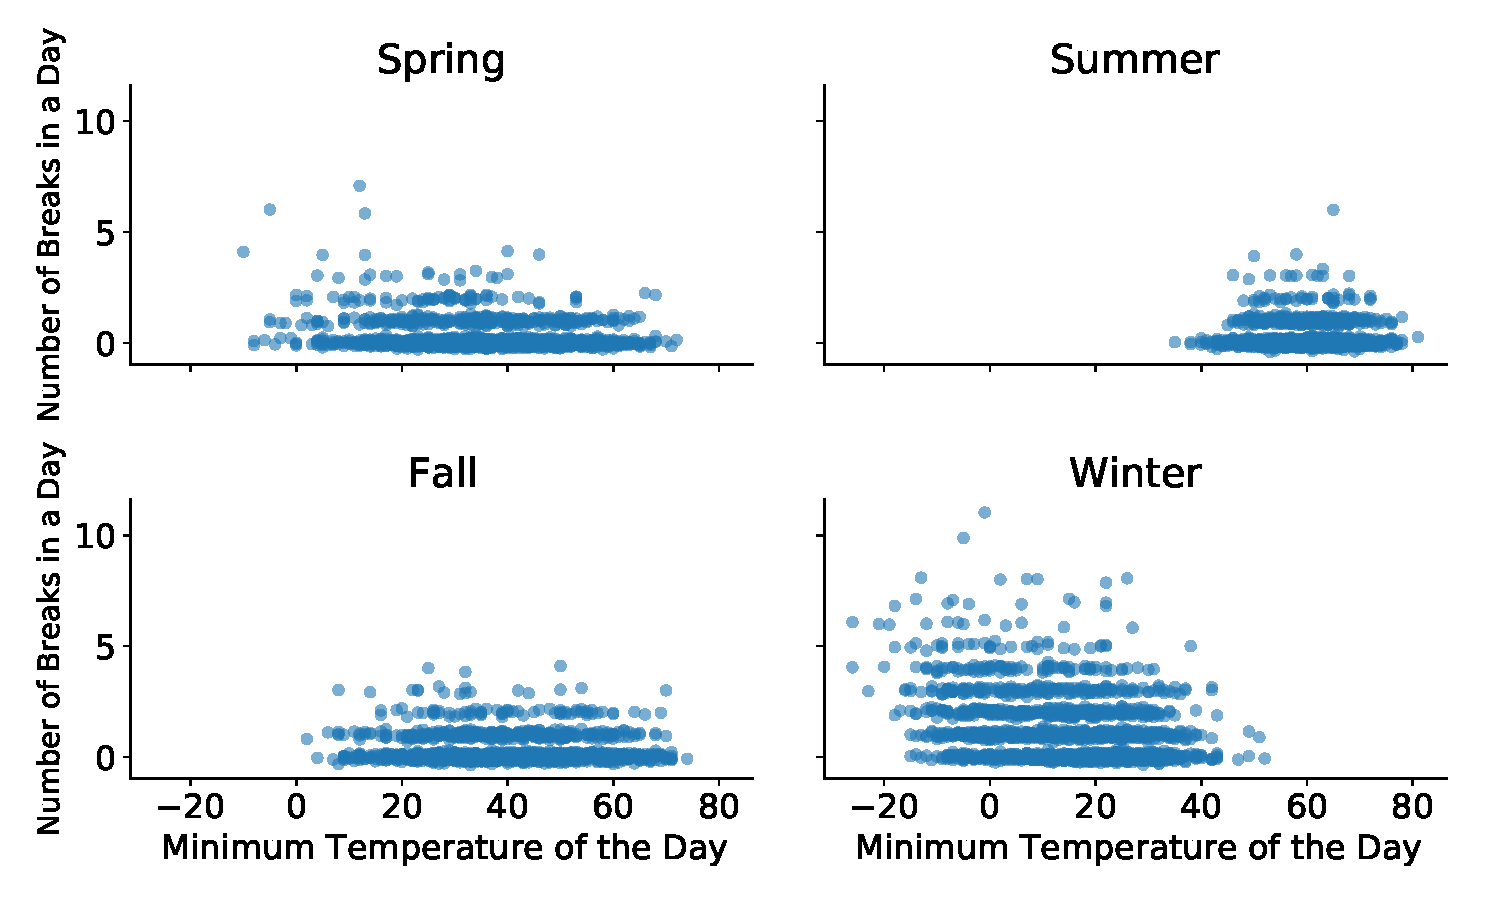
\includegraphics[width = \columnwidth]{Wen/break pattern by season.pdf}
    \caption{Number of Breakages by Soil Type categorized by Season}
    \label{fig:Break Pattern by Seaon}
\end{figure}


\subsection{Forecast}
\subsubsection{predicting breakage itself}


Figure \ref{fig:break prediction by season and temp} gives the visualization of the prediction model given the minimum temperature of a day and what season we are in. This is a second degree polynomial regression. Season is fed in using One Hot Encoding.

The minimum temperature of the day is better at predicting the number of breaks than the maximum temperature of the day by 3\% in terms of explained variance score. It makes sense because most of the breaks happen in the winter and min temperature is probably more representative of the weather that day than max temperature. We tried feeding in month of the year instead of season using One Hot Encoding and that changed the explained variance score by little. So we think splitting it into 12 months is probably too specific and season is a nice enough split. We also fed in the change in temperature from the previous day to the current day, and surprisingly, it also didn't really improve the model. In the end, it turned out that the combination of minimum temperature and season is the best at predicting the number of breaks on a given day explaining 26\% variance.

\begin{figure}[h!]
    \centering
    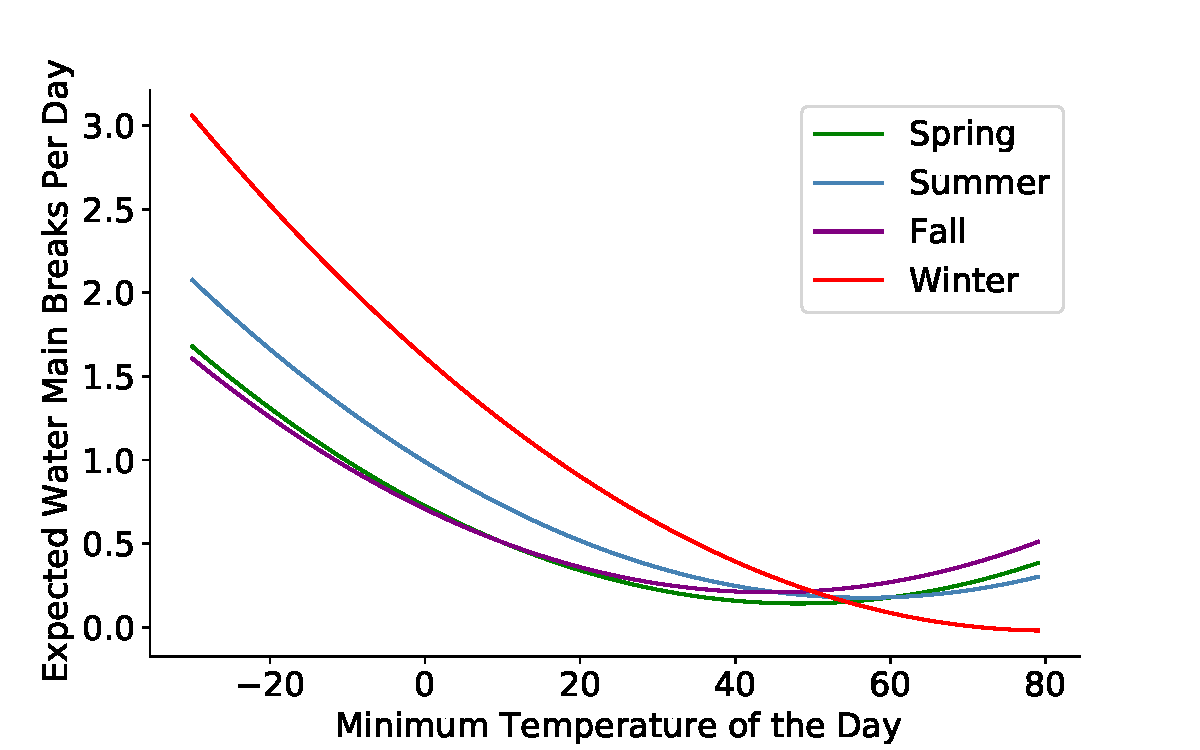
\includegraphics[width = \columnwidth]{Wen/break prediction given temperature and season.pdf}
    \caption{Prediction of the Number of Breakages given Season and Min Temp}
    \label{fig:break prediction by season and temp}
\end{figure}


\subsubsection{ predicting characteristics of breaks}

Figure \ref{fig:Polynomial Regression Total Computation} predicts of the number of breakages for different seasons of 2021 with the pipe size in metres and pipe depth in feet. Using the data on the pipe mains broken in the month of January during the past 20 years, this model forecasts the number of pipe breaks in the future years with their sizes and depths. From the figure below, we can infer that during Winter we can expect around 125 pipes to break. This will be the highest among the seasons and a majority of these pipes will be between 5 feet and 8 feet deep or between 4 metres and 8 metres long.

The figure incorporates 12 least squares regression for separate months of the year and generalizes the season resulting in increased accuracy. The features used in regression form cubic polynomials for pipe size and depth and square factors for subsequent years.   



\begin{figure}[h!]
    \centering
    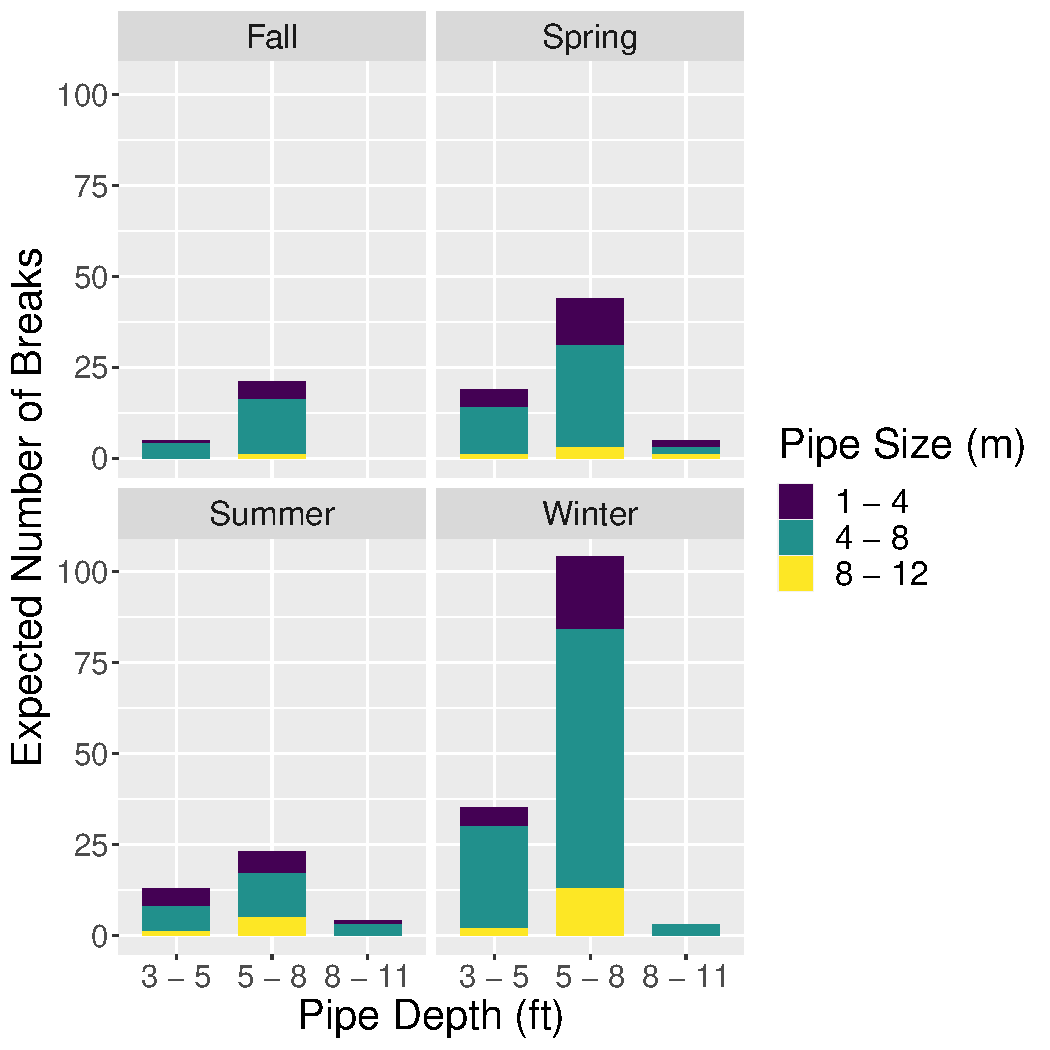
\includegraphics[scale = 0.45]{Gautam/pipemodel.pdf}
    \caption{Predicting Water Main Breaks by pipe size and depth for different seasons 2021}
    \label{fig:Polynomial Regression Total Computation}
\end{figure}



\subsubsection{Predicting the length of duration between breaks}

We also want to investigate the duration between breaks. For example, suppose a pipe main breaks and the city fixes the pipe. On average, how long will it take before the pipe breaks again? What factors influence how long the pipe can last before breaking again? 

First, we want to examine our pipe main breaks data set and analyze how often each unique pipe appears. Note that many of the pipe breaks in the data set were recorded to have occurred on January 1, 1970. This is a placeholder date. Since we are interested in duration between breaks, we filtered out the data where the date of the break was unknown. Without this placeholder date, the dates in the data set ranged from the beginning of 1997 to the beginning of 2020. 

Figure \ref{fig:num breaks} is the CDF for the distribution of the number of breaks recorded for each individual pipe in the filtered data set. The majority of pipes only have one recorded break. Of the pipes that have more than one recorded break, most pipes have 2 or 3 recorded breaks. There were a few pipes that broke over a dozen times over a 20 year span. We might investigate these pipes more thoroughly.

\begin{figure}[H]
    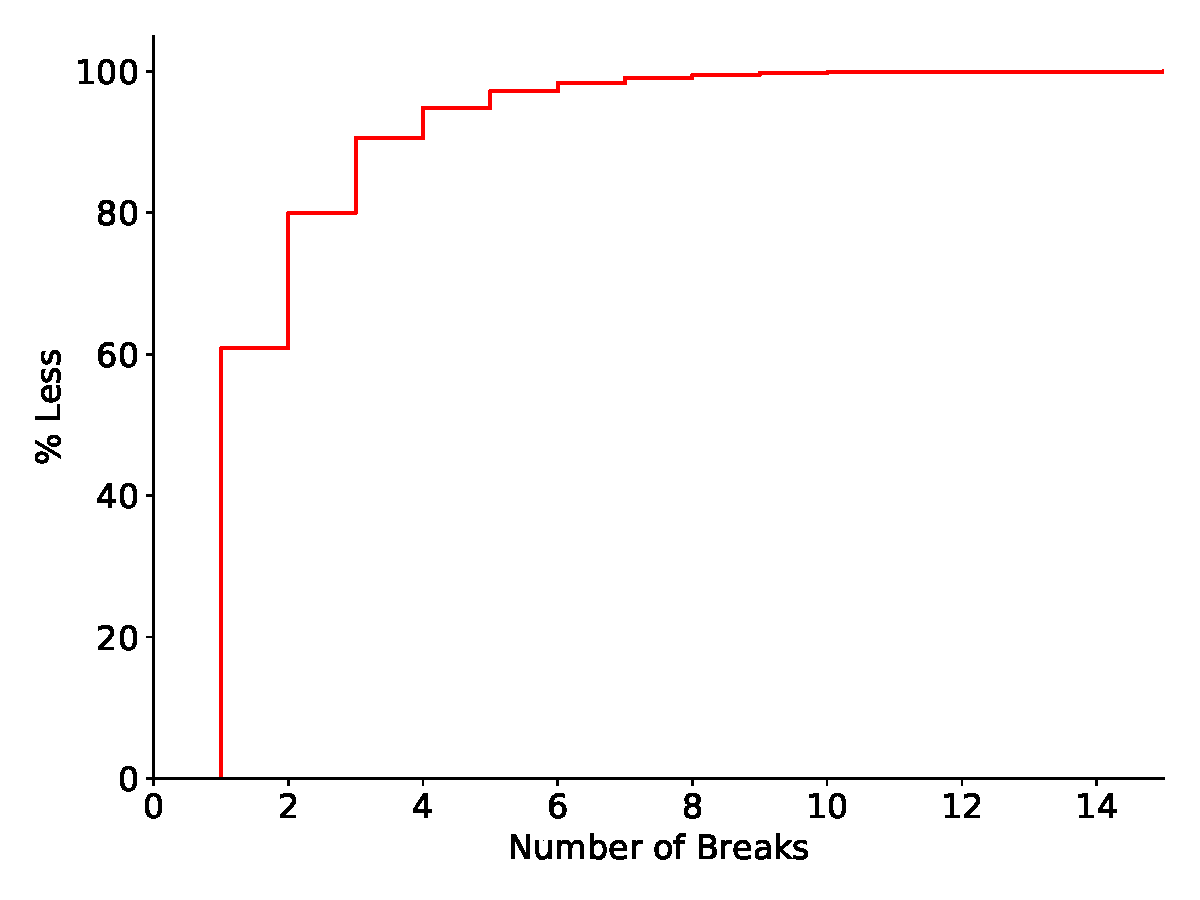
\includegraphics[width = \columnwidth]{Bryan/num_breaks.pdf}
    \caption{Number of Recorded Breaks}
    \label{fig:num breaks}
\end{figure}

For each individual pipe, we are interested in the length of the duration between the first recorded break and the second recorded break. Figure \ref{fig:first second break} is the CDF for the distribution of these duration lengths. Note that the end of the CDF does not reach 50 percent since the majority of pipes in the data set have only one recorded break. 

\begin{figure}[H]
    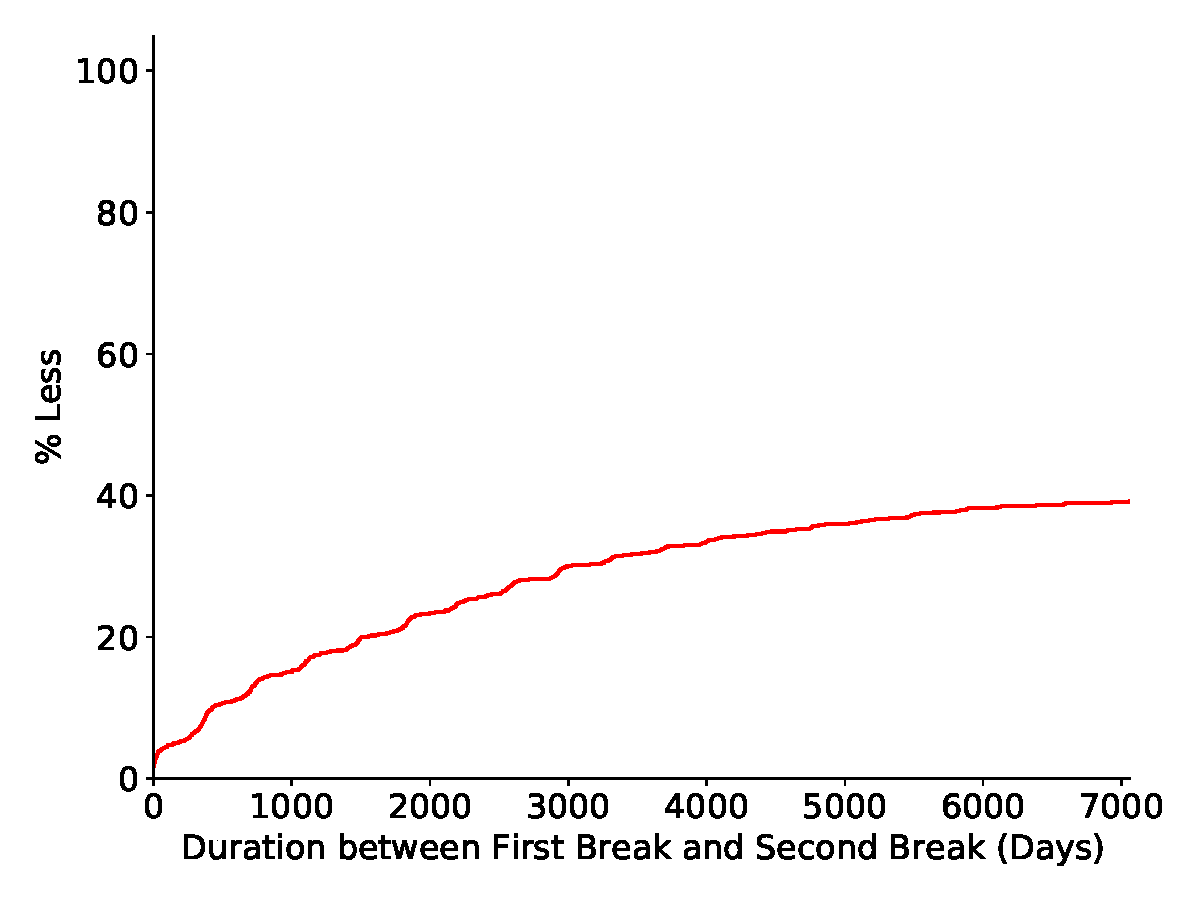
\includegraphics[width = \columnwidth]{Bryan/first_second_break.pdf}
    \caption{Time between First and Second Break}
    \label{fig:first second break}
\end{figure}

Looking at the y-intercept, we notice that some pipes actually have 0 duration between first break and second break, meaning two breaks for the same pipe on the same day were recorded in the data set. There are also pipes with two breaks differing by only one or two days. This is a strange artifact of the data set. If two breaks are recorded for the same pipe on the same day, does this actually mean the pipe was fixed and then broke again within one day? Or is this a duplicate data entry? When breaks for the same pipe differ by at most a few days, does this mean the pipe was not properly fixed? Were there some extenuating circumstances?

For now, we choose to focus on breaks that occurred at least a week apart. Figure \ref{fig:duration by year} shows, for each year, the distribution of lengths of duration between the first recorded break of a pipe and the second recorded break of a pipe. For example, suppose a pipe has its first recorded break in 2002. The second recorded break for this same pipe occurs 1500 days later. This corresponds to a point at (2002, 1500), meaning after a pipe broke for the first time on 2002, the pipe lasted 1500 days before breaking a second time. 

Note that we only look at duration lengths of at least one week and at most five years. The reason for the upper bound is that if we look at all duration lengths, including up to over 20 years, these duration lengths could only occur in the first few years. In the later years, we don't have the data to know whether longer duration lengths will be realized (we don't know what breaks will occur in the future). Therefore, we can only look at pipes where the second break didn't occur too long after the first break.

Note that for three years, 2004-2006, we see very few points. We will investigate this further. Is this because very few pipes broken during these three years? If so, why? 

\textbf{[BEGIN Bryan 11/16]}

We tried to model the length of time between the first time a pipe breaks and the second time a pipe breaks. First, we tried using year of the first break, pipe depth, season during which the first break occurred, and whether rock was present in the soil type. Unfortunately, a linear regression model suggested that none of these input variables had a statistically significant effect (using a typical alpha level of 0.05) on the length of time between first and second break. 

Figure \ref{fig:duration by year} visually shows why this is the case. Although we can see certain patterns, such as the fact that most pipes break during winter and pipe depth was only recorded starting around 2008, no variable helps explain the duration between first break and second break.

\begin{figure}[h!]
   \centering
    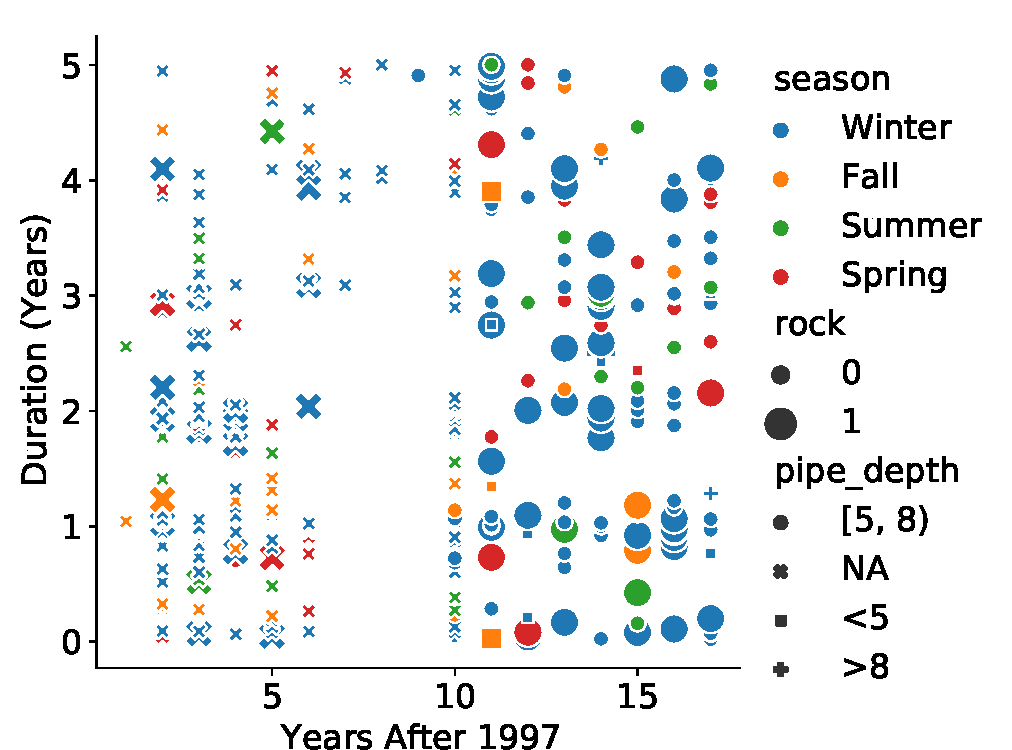
\includegraphics[scale = 0.5]{Bryan/model_fail.pdf}
    \caption{Second Breaks that came 1 Week to 5 Years after First Break}
    \label{fig:duration by year}
\end{figure}

Next, we tried to use different input variables: pipe installation year and pipe material. We thought these variables might be effective since our research suggested that more modern pipes that use DI instead of CI would be more durable. However, our linear regression model again suggested that none of our input variables had a statistically significant effect (using a typical alpha level of 0.05). 

Figure \ref{fig:duration by install year} plots the duration lengths against installation year, while figure \ref{fig:duration by material} plots the duration lengths against the pipe material. No clear pattern emerges. Although visually it looks like DI might lead to more durable pipes than CI or SPUN, a Student's t-test revealed no statistically significant difference. 

\begin{figure}[h!]
   \centering
    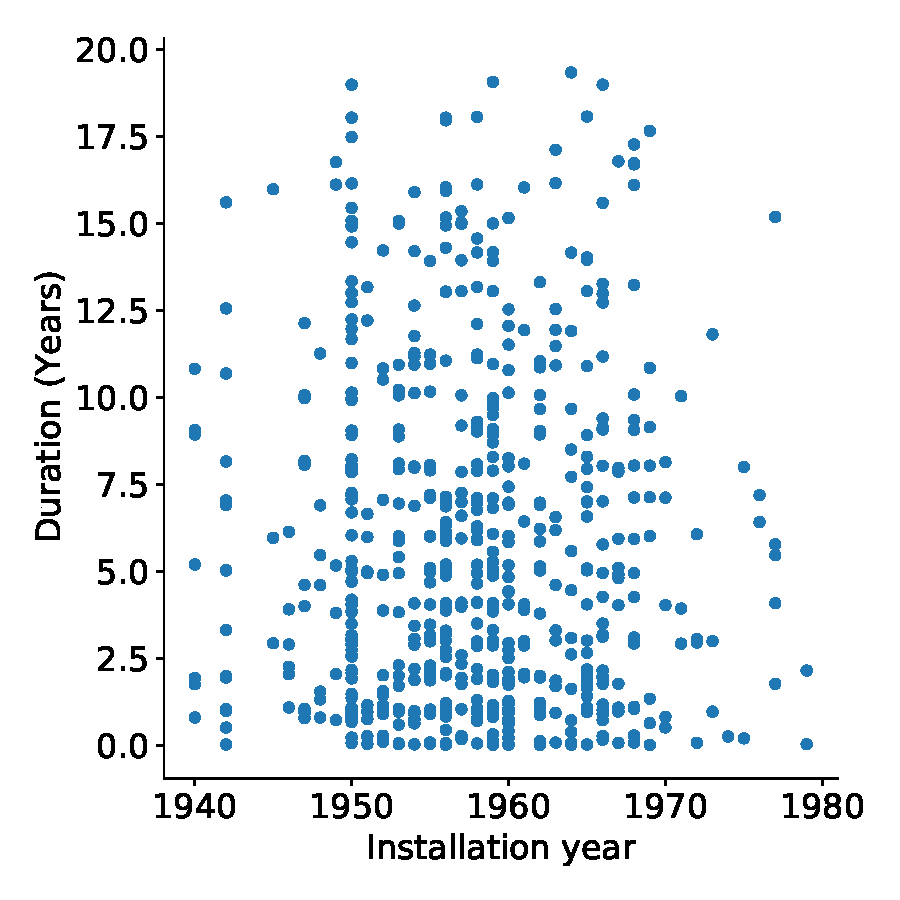
\includegraphics[scale = 0.5]{Bryan/duration_installyear.pdf}
    \caption{Length of Duration vs. Installation Year}
    \label{fig:duration by install year}
\end{figure}

\begin{figure}[h!]
   \centering
    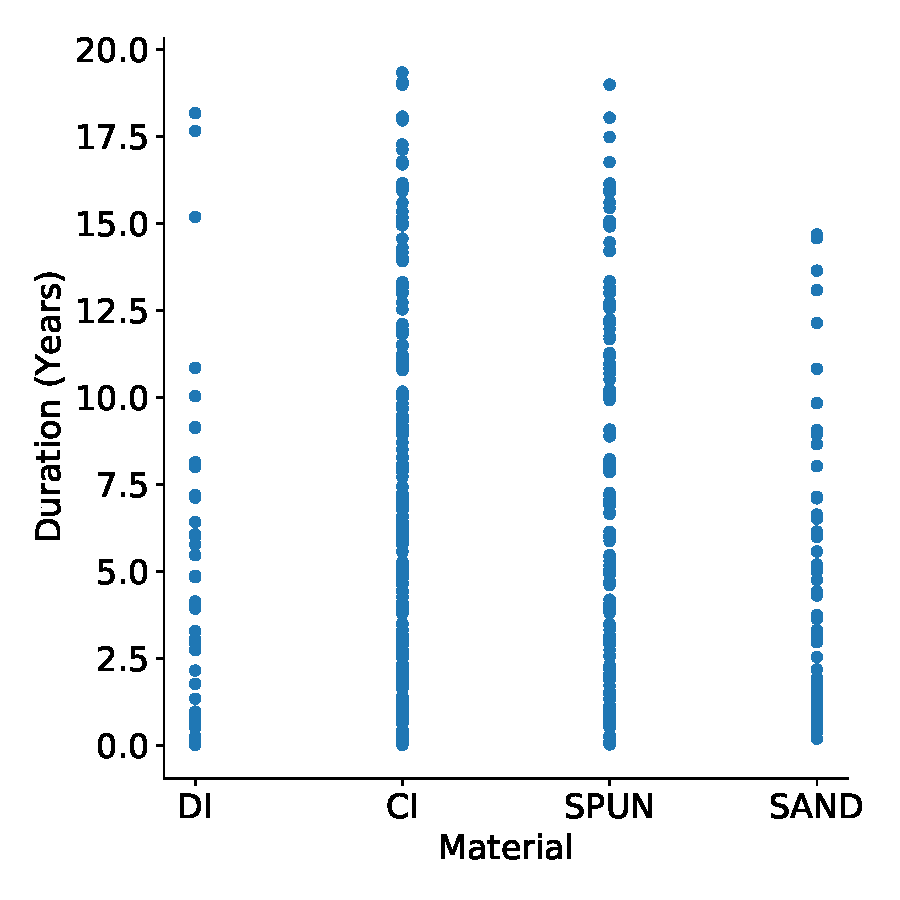
\includegraphics[scale = 0.5]{Bryan/duration_material.pdf}
    \caption{Length of Duration vs. Material}
    \label{fig:duration by material}
\end{figure}
\textbf{[END Bryan]}
\section{Final Model}



\subsection{Principal Component Analysis of Different Model Features}

\subsubsection{Material}

\textbf{[BEGIN Gautam 11/16]}

Information on the Material Data is initially found to be categorical and PCA is applied on the one hot encoded version of the Material Data. Figure \ref{fig:Material PCA} gives the principal component composition.

This is done to find a numerical equivalent to the categorical data. The weights of the first principal component shall now be used as input Material data.

\begin{figure}
    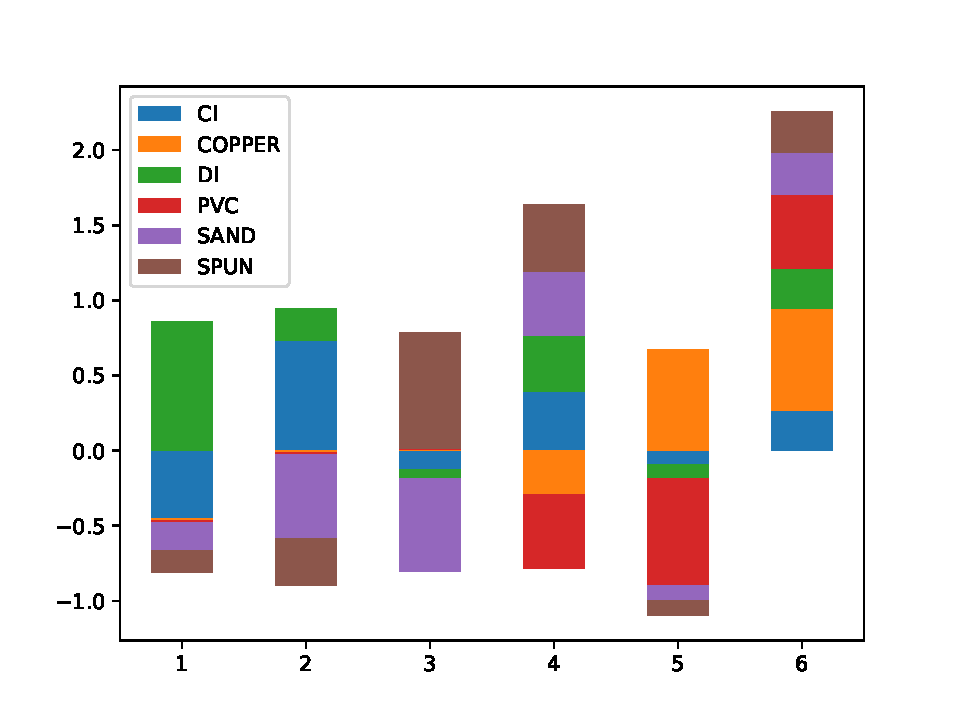
\includegraphics[width=\columnwidth]{Gautam/mat.pdf}
    \caption{Lifetime for pipes of each material}
    \label{fig:Material PCA}
\end{figure}
\textbf{[END Gautam]}




\subsubsection{Material, Lifetime,Month}

\textbf{[BEGIN Gautam 11/16]}

Figure \ref{fig:pca} shows data on three features of the main breaks: Lifetime, Month, and material, plotted to visualize possibility of reducing the data to one / two dimensional subspaces.

The numeral output of the first principal component of the material is used as Material data for PCA along with Month and lifetime.

The singular values comparison suggests that the ratio between the second and first singular values is greater than 0.1 while the between the third and first is lesser than 0.1.

Hence the plane formed by the first and second principal components justify the data well.



\begin{figure*}
\centering
    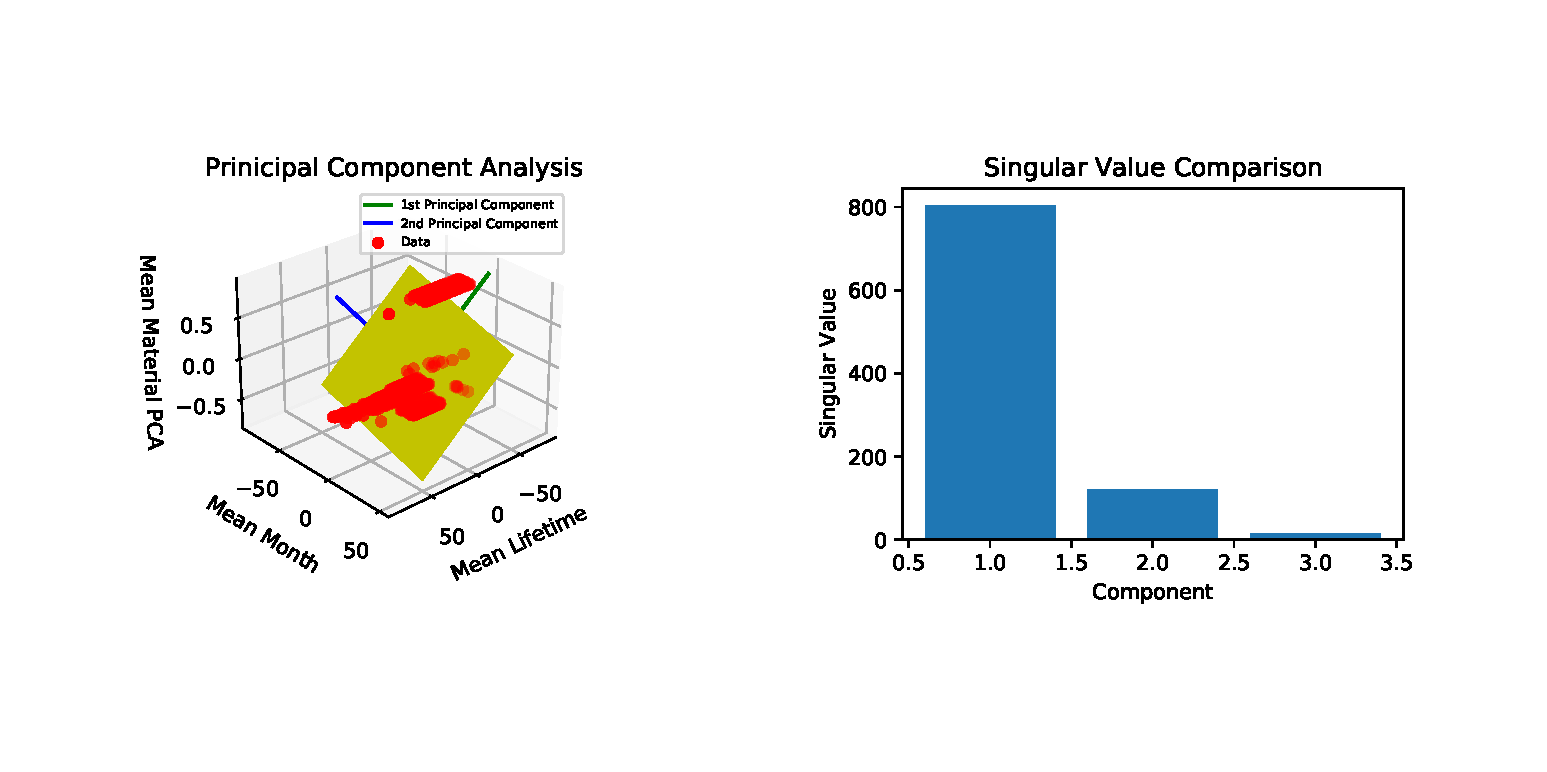
\includegraphics[width=\textwidth]{Gautam/analysis.pdf}
    \caption{Visualizing PCA of Month, Lifetime and Material}
    \label{fig:pca}
\end{figure*}

\textbf{[END Gautam]}

\section{Highlight some Conclusions}
\begin{itemize}
\item low temperatures and sudden increases in temperature cause more pipes to break
\item Season is a contributing factor to the number of breakages
\item most pipes that break are laid 5-7 feet deep and are 5-6 meters long 
\item clay and sand are primary soil types while gravel, dirt and rock are secondary soil types
\item pipes laid in gravel are more resistant to breaking during winter, and pipes laid in rock/stone are more vulnerable to breaking during winter
\end{itemize}

TODO: Full conclusion 
\end{document}
